\documentclass[12pt, a4paper]{report}

\usepackage[utf8]{inputenc}
\usepackage[T1]{fontenc}
\IfFileExists{libertine.sty}{%
  \usepackage[mono=false]{libertine}%
  \IfFileExists{zi4.sty}{\usepackage[varqu]{zi4}}{}%
}{\usepackage{lmodern}%
}
\usepackage[protrusion=true, expansion=false]{microtype}
\usepackage[a4paper, width=155mm, top=25mm, bottom=25mm, headheight=15pt]{geometry}
\usepackage{setspace}
\onehalfspacing
\emergencystretch=3em
\hbadness=2000

\usepackage{amsmath,amssymb}
\usepackage{fontawesome5}
\newcommand{\tmarkDone}{\textbf{\faCheck}}
\newcommand{\tmarkNo}{\textbf{\faTimes}}
\newcommand{\tmarkPartial}{\faHourglassHalf}
\newcommand{\tmarkPlanned}{\textcolor{black!55}{\faCircle}}
\usepackage{graphicx}
% Figures: Diagrams/ (LaTeX includes .pdf; .svg sources kept alongside for editing).
\newcommand*{\ThesisDiagDir}{Diagrams/}
\graphicspath{{Diagrams/}}
\pdfimageresolution=300
\makeatletter
\newcommand*{\@thesis@doinclude}[2]{%
  \if\relax\detokenize{#1}\relax
    \includegraphics{#2}%
  \else
    \includegraphics[#1]{#2}%
  \fi
}
\newcommand*{\@thesismissingimg}[1]{%
  \fbox{\parbox{0.92\linewidth}{\scriptsize\centering\ttfamily Missing file: \detokenize{#1}.\\[2pt]Add it to the \texttt{Diagrams/} folder and recompile.}}%
}
\newcommand{\ThesisIncludeGraphics}[2][]{%
  \IfFileExists{\ThesisDiagDir#2}{%
    \@thesis@doinclude{#1}{\ThesisDiagDir#2}}{%
  \IfFileExists{#2}{%
    \@thesis@doinclude{#1}{#2}}{%
    \@thesismissingimg{#2}%
  }}%
}
\makeatother
\newcommand{\TableScreenshotEnd}[2][]{%
  \refstepcounter{table}%
  \if\relax\detokenize{#1}\relax\else\label{#1}\fi%
  \phantomsection%
  \addcontentsline{lot}{table}{\protect\numberline{\thetable}#2}%
}
\usepackage[table]{xcolor}
\usepackage{tikz}
\usetikzlibrary{arrows.meta,positioning,fit,shapes.geometric,calc}
\usepackage{pgfplots}
\usepgfplotslibrary{statistics}
\pgfplotsset{compat=1.18, minor tick num=0}

\usepackage{booktabs}
\usepackage{array}
\usepackage{colortbl}
\usepackage{multirow}
\usepackage{float}
\usepackage{etoolbox}
\usepackage{caption}
\captionsetup{
    labelfont={bf,small},
    textfont={small},
    skip=6pt,
    format=hang
}
\makeatletter
% Compact, professional List of Figures / List of Tables (no tocloft dependency)
\renewcommand*\l@figure{\@dottedtocline{1}{0em}{3.2em}}
\renewcommand*\l@table{\@dottedtocline{1}{0em}{3.8em}}
\makeatother

\newlength{\ThesisTableImgReserve}
\newlength{\ThesisFigImgReserve}
\setlength{\ThesisTableImgReserve}{\dimexpr2\intextsep+0.75\baselineskip\relax}
\setlength{\ThesisFigImgReserve}{\dimexpr2\intextsep+\abovecaptionskip+\belowcaptionskip+4\baselineskip\relax}
\newcommand{\TableImageMaxFit}[1]{%
  \ThesisIncludeGraphics[
    width=0.7\linewidth,
    height=\dimexpr(\textheight-\ThesisTableImgReserve)*7/10\relax,
    keepaspectratio
  ]{#1}%
}
\newcommand{\FigureImageMaxFit}[1]{%
  \ThesisIncludeGraphics[width=\linewidth,height=\dimexpr\textheight-\ThesisFigImgReserve\relax,keepaspectratio]{#1}%
}
\newcommand{\OnePageDiagram}[2][]{%
  \if\relax\detokenize{#1}\relax
    \ThesisIncludeGraphics[width=\linewidth,height=\dimexpr\textheight-\ThesisFigImgReserve\relax,keepaspectratio]{#2}%
  \else
    \ThesisIncludeGraphics[#1,width=\linewidth,height=\dimexpr\textheight-\ThesisFigImgReserve\relax,keepaspectratio]{#2}%
  \fi
}
\newcommand{\HalfWidthDiagram}[1]{%
  \ThesisIncludeGraphics[width=0.5\linewidth, keepaspectratio]{#1}%
}
\newcommand{\WideDiagram}[2][]{%
  \if\relax\detokenize{#1}\relax
    \ThesisIncludeGraphics[width=\linewidth, height=0.78\textheight, keepaspectratio]{#2}%
  \else
    \ThesisIncludeGraphics[#1, width=\linewidth, height=0.78\textheight, keepaspectratio]{#2}%
  \fi
}
\newcommand{\TallDiagram}[2][]{%
  \if\relax\detokenize{#1}\relax
    \ThesisIncludeGraphics[width=\linewidth, height=0.96\textheight, keepaspectratio]{#2}%
  \else
    \ThesisIncludeGraphics[#1, width=\linewidth, height=0.96\textheight, keepaspectratio]{#2}%
  \fi
}
% Balanced layout slot (reference: Figure 4.3 ml-explainability) — wide banded diagrams.
\newcommand{\BalancedDiagram}[2][]{%
  \if\relax\detokenize{#1}\relax
    \ThesisIncludeGraphics[width=\linewidth, height=0.72\textheight, keepaspectratio]{#2}%
  \else
    \ThesisIncludeGraphics[#1, width=\linewidth, height=0.72\textheight, keepaspectratio]{#2}%
  \fi
}
% Activity diagrams — full-height slot for 3× label size.
\newcommand{\ActivityDiagram}[2][]{%
  \if\relax\detokenize{#1}\relax
    \ThesisIncludeGraphics[width=\linewidth, height=\textheight, keepaspectratio]{#2}%
  \else
    \ThesisIncludeGraphics[#1, width=\linewidth, height=\textheight, keepaspectratio]{#2}%
  \fi
}
% Half-size slot (50\% of BalancedDiagram width and height).
\newcommand{\CompactDiagram}[2][]{%
  \if\relax\detokenize{#1}\relax
    \ThesisIncludeGraphics[width=0.5\linewidth, height=0.36\textheight, keepaspectratio]{#2}%
  \else
    \ThesisIncludeGraphics[#1, width=0.5\linewidth, height=0.36\textheight, keepaspectratio]{#2}%
  \fi
}
\usepackage[skins]{tcolorbox}
% Empty slot for figures pending vector artwork (no PNG in thesis).
\newcommand{\FigurePlaceholder}[1][0.72\textheight]{%
  \begin{tcolorbox}[colback=white,colframe=gray!35,boxrule=0.4pt,arc=0pt,
    width=\linewidth,height=#1,halign=center,valign=center]
    \mbox{}
  \end{tcolorbox}
}

\usepackage{titlesec}
\usepackage{parskip}
\usepackage{fancyhdr}
\usepackage{enumitem}
\PassOptionsToPackage{hyphens,spaces,obeyspaces}{url}
\usepackage{hyperref}
\makeatletter
\g@addto@macro\UrlBreaks{\do\/\do\-\do\.\do\:\do\&\do\=\do\#}
\makeatother

\definecolor{PrimaryBlue}{HTML}{000000}
\definecolor{AccentBlue}{gray}{0.55}
\definecolor{LightBlue}{gray}{0.96}
\definecolor{MidBlue}{gray}{0.90}
\definecolor{DarkText}{HTML}{000000}
\definecolor{GrayText}{gray}{0.45}
\definecolor{RowShade}{gray}{0.965}
\definecolor{RowShadeAlt}{gray}{0.92}
\definecolor{TableHeadBg}{gray}{0.88}
\definecolor{TableRule}{gray}{0.55}
\definecolor{GreenAccent}{HTML}{000000}
\definecolor{AmberAccent}{HTML}{000000}
\definecolor{RedAccent}{HTML}{000000}
\definecolor{VioletAccent}{HTML}{000000}

\hypersetup{
    colorlinks=true,
    linkcolor=black,
    filecolor=black,
    urlcolor=black,
    citecolor=black,
    pdfborder={0 0 0},
}

\titleformat{\chapter}[display]
    {\normalfont\LARGE\bfseries}
    {\chaptertitlename\ \thechapter}{20pt}{\LARGE}
    [\vspace{4pt}{\color{black!40}\titlerule[0.6pt]}]

\titleformat{\section}
    {\large\bfseries}
    {\thesection}{0.8em}{}

\titleformat{\subsection}
    {\normalsize\bfseries}
    {\thesubsection}{0.6em}{}

\titleformat{\subsubsection}
    {\normalsize\bfseries\itshape}
    {\thesubsubsection}{0.6em}{}

\titlespacing*{\chapter}{0pt}{-20pt}{20pt}
\titlespacing*{\section}{0pt}{16pt plus 3pt minus 2pt}{8pt plus 2pt minus 1pt}
\titlespacing*{\subsection}{0pt}{12pt plus 2pt minus 1pt}{6pt plus 1pt minus 1pt}
\titlespacing*{\subsubsection}{0pt}{10pt plus 2pt minus 1pt}{4pt plus 1pt minus 1pt}

\newcommand{\tableheadcolor}{\rowcolor{TableHeadBg}}
\newcommand{\tableheadfont}{\bfseries}
\newcommand{\ThesisTableBodyFont}{\small}

% Consistent greyscale table polish (font size unchanged; spacing only).
\newcommand{\ThesisTablePrep}{%
  \ThesisTableBodyFont
  \renewcommand{\arraystretch}{1.22}%
  \setlength{\tabcolsep}{6pt}%
  \arrayrulecolor{TableRule}%
  \setlength{\aboverulesep}{0.55ex}%
  \setlength{\belowrulesep}{0.55ex}%
}
\AtBeginEnvironment{table}{\ThesisTablePrep}
\AtBeginEnvironment{tabular}{%
  \rowcolors{2}{}{RowShade}%
  \arrayrulecolor{TableRule}%
}

\newenvironment{moderntable}[1][H]{%
    \begin{table}[#1]\centering\ThesisTablePrep
}{%
    \end{table}%
}

\newtcolorbox{layerbox}[1]{
    colback=white,
    colframe=black!55,
    coltitle=black,
    fonttitle=\bfseries\small,
    title=#1,
    boxrule=0.6pt,
    arc=2pt,
    left=6pt,right=6pt,top=4pt,bottom=4pt,
}

\newtcolorbox{highlightbox}[1][]{
    colback=black!4,
    colframe=black!45,
    boxrule=0.5pt,
    arc=2pt,
    left=8pt,right=8pt,top=6pt,bottom=6pt,
    #1
}

\newtcolorbox{chapterinstruction}[2][]{%
  colback=black!4,colframe=black!55,title={#2},fonttitle=\bfseries\small,
  arc=2pt,left=8pt,right=8pt,top=6pt,bottom=6pt,#1}

\pagestyle{fancy}
\fancyhf{}
\renewcommand{\headrulewidth}{0.4pt}
\fancyhead[L]{\small\color{black!55}Crypto World Bank}
\fancyhead[R]{\small\color{black!55}BRAC University}
\fancyfoot[C]{\small\color{black!55}\thepage}

\begin{document}

%% ============================================================
%% TITLE PAGE
%% ============================================================
\thispagestyle{empty}

\begin{center}

\vspace*{0.3cm}

\ThesisIncludeGraphics[width=3.5cm]{bracu_logo_12-0-2022.pdf}

\vspace{0.8cm}

{\LARGE\bfseries\color{PrimaryBlue} Decentralized Crypto World Bank}\\[0.4em]
{\large\color{PrimaryBlue!80} A Blockchain-Based Lending Platform\\[0.15em]with AI-Enhanced Security}

\vspace{0.6cm}

{\normalsize\bfseries Thesis ID: [P26101123]}

\vspace{1.2cm}

{\large by}

\vspace{0.5cm}

{\Large\bfseries\color{PrimaryBlue} Md.\ Bokhtiar Rahman Juboraz}\\[0.2em]
{\color{GrayText}20301138}\\[0.8em]
{\Large\bfseries\color{PrimaryBlue} Md.\ Mahir Ahnaf Ahmed}\\[0.2em]
{\color{GrayText}20301083}

\vspace{1.2cm}

A pre-thesis 1 report submitted to the Department of Computer Science and Engineering\\
in partial fulfillment of the requirements for the degree of\\
\textbf{B.Sc.\ in Computer Science}

\vfill

{\color{PrimaryBlue}\rule{0.4\textwidth}{0.6pt}}\\[0.6em]
Department of Computer Science and Engineering\\
\textbf{BRAC University}\\
February 2026

\vspace{0.5cm}

{\small\color{GrayText}\copyright\ 2026.\ BRAC University --- All rights reserved.}

\end{center}

%% ============================================================
%% DECLARATION
%% ============================================================
\newpage
\thispagestyle{empty}

\chapter*{Declaration}
\phantomsection
\addcontentsline{toc}{chapter}{Declaration}

It is hereby declared that

\begin{enumerate}
\item The report submitted is our own original work while completing degree at BRAC University.

\item The report does not contain material previously published or written by a third party, except where this is appropriately cited through full and accurate referencing.

\item The report does not contain material which has been accepted, or submitted, for any other degree or diploma at a university or other institution.

\item We have acknowledged all main sources of help.
\end{enumerate}

\vspace{2cm}

\textbf{Student's Full Name \& Signature:}

\vspace{0.8cm}

\noindent
\begin{minipage}[t]{0.42\textwidth}
\centering
\ThesisIncludeGraphics[width=2.1cm,keepaspectratio]{bokhtiar-sign.pdf}\\[0.5cm]
Md. Bokhtiar Rahman Juboraz\\[0.2cm]
20301138
\end{minipage}\hfill
\begin{minipage}[t]{0.42\textwidth}
\centering
\ThesisIncludeGraphics[width=2.1cm,keepaspectratio]{mahir-sign.pdf}\\[0.5cm]
Md. Mahir Ahnaf Ahmed\\[0.2cm]
20301083
\end{minipage}

%% ============================================================
%% APPROVAL
%% ============================================================
\newpage
\thispagestyle{empty}

\chapter*{Approval}
\phantomsection
\addcontentsline{toc}{chapter}{Approval}

The pre-thesis 1 report of final year project titled ``Decentralized Crypto World Bank: A Blockchain-Based Lending Platform with AI-Enhanced Security'' submitted by

\begin{enumerate}
\item Md. Bokhtiar Rahman Juboraz (20301138)
\item Md. Mahir Ahnaf Ahmed (20301083)
\end{enumerate}

Of Spring, 2026 has been accepted as satisfactory in partial fulfillment of the requirement for the degree of B.Sc. in Computer Science on February 20, 2026.

\vspace{1cm}

\textbf{Examining Committee:}

\vspace{1.5cm}

\begin{flushleft}
Supervisor:\\
(Member)
\end{flushleft}

\begin{flushright}
\vspace{-0.5cm}
\hrulefill\\
Mr. Annajiat Alim Rasel\\
Senior Lecturer\\
Department of Computer Science and Engineering\\
BRAC University
\end{flushright}

\vspace{1.5cm}

\begin{flushleft}
Project Coordinator:\\
(Member)
\end{flushleft}

\begin{flushright}
\vspace{-0.5cm}
\hrulefill\\
Dr. Md. Golam Rabiul Alam\\
Professor\\
Department of Computer Science and Engineering\\
BRAC University
\end{flushright}

\newpage
\thispagestyle{empty}

\null\vfill

\begin{flushleft}
Head of Department:\\
(Chair)
\end{flushleft}

\begin{flushright}
\vspace{-0.5cm}
\hrulefill\\
Dr. Sadia Hamid Kazi\\
Chairperson and Associate Professor\\
Department of Computer Science and Engineering\\
BRAC University
\end{flushright}

\vfill\null

%% ============================================================
%% ETHICS STATEMENT
%% ============================================================
\newpage
\thispagestyle{empty}

\chapter*{Ethics Statement}
\phantomsection
\addcontentsline{toc}{chapter}{Ethics Statement}

This project is designed to be functional on public blockchain testnets, with no intention for monetary profit, nor to create institutional leverage over decentralized financing. No personal banking data, or private financial data, or codes of existing projects, are used in the development of the prototype platform and training AI/ML data. The full project prototype build is to be demonstrated in the final defence of the project; the platform is expected to be ready for testing and troubleshooting by pre-thesis~2. All the development workflow can be traced by the official GitHub repository for the project, and the planning, coding, testing, and usage of different dependencies for this project is considered open-source with MIT licensing, and will be open for contribution after the submission of the final build. For the training of the AI models, AI-assisted financial decision-making, risk assessment, privacy features, on-chain and off-chain data processing and data storing, we acknowledge the ethical considerations while making decisions for the development of the project.

%% ============================================================
%% ABSTRACT
%% ============================================================
\newpage
\thispagestyle{empty}

\chapter*{Abstract}
\phantomsection
\addcontentsline{toc}{chapter}{Abstract}

In the modern world, global financing relies on institutional structures that are multilayered and complex that extend throughout the borders of nations, adapting complex protocols to maintain balance in the economy; however, these systems often struggle to maintain transparency and equal access to credit across the world. Decentralized financing has improved transparency in financing by adapting programmable infrastructures that can automate exchanges or structured governance, but the existing models use mostly flat architecture that does not match with the traditional institutional hierarchies or governance that is well structured based on global economic contexts. This creates a scope to study and explore how tier-based financial systems that mimic the functionalities, but in a decentralized environment with the flexibility and adaptability. As an attempt to address this opportunity and to demonstrate what is possible, we present our research-based project \textit{Crypto World Bank}, a formally specified prototype which is based on blockchain-based institutional finance, that includes coordinating capital allocation across multi-tiered hierarchical governance structures. The primary focus of the project is a smart-contract that includes a hierarchy with a pipeline of oracle-based risk-analytics (Random Forest, Isolation Forest, SHAP, which will be trained and benchmarked with existing similar systems); an optional intelligent MCP agent as a feature to interact with the UI with more comfort, while all the core banking systems remain intact by using wallets. The banking architecture includes risk intermediation, liquidity management, deposit mobilization, credit allocation, payment settlement, and other adjacent financial services. The development workflow including frontend, smart contract, oracle integration and overall system architecture and design is specified in this paper; implementation and testnet deployment are planned across four phases in the final stages. The goal of this project paper is to illustrate how a hybrid system of design of decentralized system can converge with institutional systems, to set a foundation for research on how a hierarchically governed crypto financial system can be developed.

\vspace{0.5em}
\noindent\textbf{Keywords:} Blockchain, Decentralized Finance, Deposit Mobilization, Explainable AI, Financial Sustainability, Group Lending, Hierarchical Lending, Institutional DeFi, Multi-Entity Co-Lending, Oracle-Mediated Risk Analytics, Reserve Management, Smart Contracts

%% ============================================================
%% DEDICATION
%% ============================================================
\newpage
\thispagestyle{empty}

\chapter*{Dedication}
\phantomsection
\addcontentsline{toc}{chapter}{Dedication}

\vspace{3cm}
\begin{center}
\textit{Dedicated to our families for their unwavering support throughout our academic journey.}
\end{center}

%% ============================================================
%% ACKNOWLEDGMENT
%% ============================================================
\newpage
\thispagestyle{empty}

\chapter*{Acknowledgment}
\phantomsection
\addcontentsline{toc}{chapter}{Acknowledgment}

We would like to express our sincere gratitude to our panel members for their guidance and support throughout this project. We also thank our supervisor, Mr.\ Annajiat Alim Rasel, Senior Lecturer at the Department of Computer Science and Engineering, BRAC University, for his guidance and support. Finally, we thank the Department of Computer Science and Engineering at BRAC University for providing us with the resources and academic environment to pursue this work.

%% ============================================================
%% TABLE OF CONTENTS
%% ============================================================
\newpage
\singlespacing
\setcounter{page}{1}
\pagenumbering{roman}
\tableofcontents
\newpage
\listoffigures
\newpage
\listoftables
\newpage
\pagenumbering{arabic}
\setcounter{page}{1}

\chapter{Introduction}
\label{sec:intro}

The \textit{Crypto World Bank} is a research-based project for exploring how blockchain technology can be shaped to fit into institutional financial systems with all the added benefits that come with a decentralized financing system. Based on our findings that had similar motivation to our study, existing DeFi protocols show isolated functionalities, such as Aave for lending, Uniswap for exchange, and MakerDAO for stablecoins. This project specifies a tier-based, hierarchically governed platform that includes a mixture of institutional financing with DeFi, accommodating deposit mobilization, credit allocation, interbank liquidity, installment repayment, FX facilitation, solidarity group lending, reserve enforcement, syndicated co-lending, and risk-based governance covering all four tiers that systematically mirrors real-world institutional financing. At the top, Tier~1 represents the World Bank reserve; the core banking hierarchy is specified in Solidity and being improved until final deployment. Another significant feature---the multi-entity contract suite---is fully specified in Chapter~3, which is scheduled for practical development in Phases~II--III.

The system is designed for three categories of participant: a programmable World Bank reserve as Tier~1, national and local development banks serving in Tiers~2--3, and retail clients in Tier~4. Retail clients get access to savings, group loans, and installment lending features. This hierarchical structure in this project was motivated by unbanked and MSME financing gaps~[9, 11]. The project is not built with any motivation to deploy only in regions with access to advanced technologies; rather, proper distribution of access to finance and fairness is the leading cause of this attempt to find suitable ground to adapt DeFi among the general population. The whole project is open source and available in our \href{https://github.com/Yuvraajrahman/Cryto-World-Bank}{GitHub repository}. The added benefits of blockchain: it provides state visibility, tamper-evident audit trails, and programmable rule enforcement among institutions having competition, as demonstrated by the renowned World Bank FundsChain programme~[27] and JPMorgan Kinexys~[28]. From the study of institutions, open ledger infrastructure and institutional hierarchy are not mutually exclusive.

\begin{figure}[H]
\centering
\BalancedDiagram{Ch1_system-overview-four-tier-stack.pdf}
\caption[Crypto World Bank system overview]{Crypto World Bank system overview}
\label{fig:intro-system-overview}
\end{figure}

\section{Background}
\label{sec:background}

Local lenders, or our target users, for this aspect of lending through layered institutions---supranational bodies that is provided by development finance channels have structural costs. Idle capital is usually locked by correspondent banking in pre-funded nostro/vostro accounts~[14], cross-border transactions that take around two to five days cost roughly \$45 per transaction~[15], charges for remittance corridors average 6.49\%, which is above the UN SDG target of 3\%~[16]. Due to unequal access to traditional banking systems, 1.4~billion adults remain unbanked~[9] and MSMEs face a \$4.5~trillion annual financing gap~[11].

In decentralized financing, lending, collateral, and interest can be automated by enabling rules on-chain transparently. However, institutions like Aave~v3 that holds \$26.3~billion TVL~[17] and the broader DeFi lending market exceeds \$55~billion~[8], use flat pool design that ignore institutional hierarchy, inter-tier exchange, and accessing clients via local bank lend path which is more generalized for normal people with less knowledge about DeFi.

\paragraph{Contribution of smart-contract and blockchain.}
Smart-contracts can develop lending rules as immutable, atomic, with auditable on-chain logic. This technology replaces the bilateral ledger reconciliation with a system of shared record, when a local bank initiates a loan, the World Bank's reserve ratio updates on the same transaction status~[27]. DeFi extends this feature to financial services without licensed custodians. Here in The \textit{Crypto World Bank} adds three dimensional feature that is missing from the existing institutional protocols: institutional hierarchy (four-tier capital flows), multi-entity operations (solidarity groups, syndicated loans, tranched pools), and a connection to the evolving development finance framework identified as absent in the literature~[1].

\paragraph{Optional conversational interface.}
Every user interacts with this system primarily through the React UI and wallet credential signing. For development purposes and demonstration, a locally hosted agent (Qwen3-8B + MCP, 17 banking tools) provides an alternate path to get the essential tasks done, including all the customer services that require system interaction information guidance and assistance in acquiring a loan or exchange finances with the system. In the final build it is planned to be replaced with secured API-based services.

\paragraph{Technical foundations.}
\label{sec:blockchain-fundamentals}

\textbf{Consensus.} The chain is an append-only ledger: nodes agree on history, and no one can rewrite past blocks without controlling most of the network~[50].

\textbf{EVM execution~[41].} Loan logic runs as deterministic bytecode on Ethereum-compatible chains. Storage writes are the main cost driver (Section~\ref{sec:gas-cost}).

\textbf{State machines.} Each loan moves through clear stages---\texttt{PENDING} $\to$ \texttt{APPROVED} $\to$ \texttt{ACTIVE} $\to$ \texttt{REPAYING} $\to$ \texttt{COMPLETED/DEFAULTED}---with only authorised roles allowed to advance it.

\textbf{Oracles~[45, 76].} Contracts cannot read off-chain data on their own. ML risk scores reach the chain via a commit-reveal oracle (Section~\ref{sec:oracle-architecture}); Chainlink Feeds, Automation, and Proof of Reserve handle prices, due-date checks, and reserve attestation. Live ML wiring starts after pre-thesis~2.

\textbf{Polygon zkEVM.} We deploy on Cardona testnet (Section~\ref{sec:high-level-arch}) for low fees and L1-backed validity proofs.

\section{Rationale and Motivation}
\label{sec:rationale}

Real development finance depends on layered institutions, yet settlement friction, opaque reserves, and correspondent-banking idle capital leave both intermediaries and unbanked clients underserved~[16, 90]. Flat DeFi protocols automate lending at scale but ignore institutional hierarchy, cross-tier flows, and the Local-Bank-to-client path that microfinance and development banks use in practice~[1]. This study is motivated by the opportunity to encode that hierarchy on a programmable ledger---with enforced reserves, role-based governance, and auditable capital movement---while supporting (not replacing) human credit judgment through lightweight analytics and an optional conversational interface. The thesis specifies a reusable architecture; it does not claim a particular national deployment target.

\section{Problem Statement}

Three primary forces of motivation for this study: development-finance has restricting transparency and settlement; the absence of multi-tiered banking functions in DeFi (deposits, solidarity and lending); the keen interest in combining blockchain auditability with ML computational analytics. There are six structural inefficiencies noticeable in development finance routes for individual borrowers from national and local banks:

\begin{enumerate}[noitemsep]
\item \textbf{Lack of transparency:} there is very little chance of the lower tier users to verify capital management, reserve levels or lending decisions are made by the higher tiers, very less transparency on how money flows through the different levels of systems. Only the top tiers get the information and records of reserves and audited at most quarterly.
\item \textbf{Sluggish settlements and idle capital:} cross-border transactions are quite expensive, average \$45 per transaction~[15], and time consuming taking two to five days~[21].
\item \textbf{Inconsistent risk evaluation:} fraud and credit assessment are completely relied on human judgement, borrowers are generally re-evaluated at each tier or institutions based on information available at that tier, no unified credit history.
\item \textbf{Access and trust barriers:} the cost of inter-institutional trust is quite expensive for legal and audit process. It creates congestions in developing countries where investors earn returns roughly 3\% below compared to developed markets~[18].
\item \textbf{No programmable savings:} depositors in developing economies have no real-time access to visibility into how savings are processed and deployed.
\item \textbf{No on-chain group credit:} without individual collateral, borrowers cannot access programmable on-chain mutual group lending with shared responsibility. Real-world organizations like BRAC exist but does not function like DeFi.
\end{enumerate}

DeFi enabled automatic lending transparency at scale such as Aave~v3 with \$26.3~billion TVL, \$17.7~billion borrows~[17], Compound~v3 (\$1.4~billion)~[19], MakerDAO with \$10.5~billion stablecoin issuance~[20]. Despite large market coverage they exhibit four limitations for institutional development finance:

\begin{itemize}[noitemsep]
\item \textbf{Flat lending models.} Aave/Compound uses one protocol for many asset pools (USDC, ETH, etc.). There is no cross-tier allocation, no institutional hierarchy, no difference in role-based governance. Here our CWB models institutional relationships that go deep into what kind of services to provide to what kind of roles/institutions to increase liquidity in overall lending and exchange situations.
\item \textbf{No AI risk analytics.} DeFi relies on collateral ratio, utilization curves. There is no behavioral fraud detection or explainable credit support system.
\item \textbf{No tiered governance.} DeFi protocol treats tokens as a measurement of voting, not based on what is the role of the client or user or institution in the bigger to smaller picture as it lacks relation to a deeper level like institutions.
\item \textbf{Single-level institutional DeFi.} Maple \& Goldfinch~[51] with \$2.6--3.8~billion TVL and \$680~million originations in 18+ countries respectively serve institutions, but none models a full multi-tier banking system with interbank flows, lack hierarchical capital flows.
\end{itemize}

\section{Objectives}

The objectives of this project are:

\begin{enumerate}[noitemsep]
\item Design and specify all features and constraints of a four-tier lending architecture on an EVM-compatible blockchain and complete a full testnet deployment (World Bank $\to$ National Bank $\to$ Local Bank $\to$ Client). The whole development cycle is planned for Phases~I--IV.
\item Design not only pool lending, but specify an extended banking product suite on the hierarchical system (deposits, savings, and solidarity group lending).
\item Investigate a lightweight off-chain analytics layer using ML, training and testing the models in practical testnet for fraud detection, anomaly detection, explainable review, and an optional MCP-based conversational interactive agent for ease of use.
\item Specify programmable on-chain lending with borrowing limits based on financial behaviour analysis, installments, and role-based access control and information via smart contracts.
\item Plan and execute testnet deployment using Polygon zkEVM Cardona, Ethereum Sepolia, and evaluate hierarchical controls in the final thesis phase.
\item Document governance for future improvements, security analysis and feature improvements, role-based regulatory considerations, and a controlled rollout toward sandbox piloting.
\end{enumerate}

\section{Proposed Solution}
\label{sec:proposed-solution}

The Crypto World Bank will implement a four-tier on-chain lending model: Tier~1 World Bank reserve custodian $\to$ Tier~2 National Banks $\to$ Tier~3 Local Banks processing retail loans $\to$ Tier~4 clients building on-chain credit history (Figure~\ref{fig:intro-system-overview}), with six standard banking functions enforced on-chain---deposit mobilization, credit allocation, payment and settlement, risk intermediation, liquidity management, and ancillary services---rather than discretionary audit alone.
\label{sec:banking-functions}
Banks also borrow from peers, park surplus with parent tiers, and syndicate large loans; the platform replicates four-tier downward flow, same-tier pools, upward deposits, and multi-bank co-funding on-chain (Figure~\ref{fig:cross-tier-lending}).
\label{sec:cross-tier-lending}

\begin{figure}[H]
\centering
\BalancedDiagram{Ch1_cross-tier-lending-flows.pdf}
\caption[Cross-tier lending flow directions]{Cross-tier lending flow directions}
\label{fig:cross-tier-lending}
\end{figure}

\paragraph{Can a group of entities lend or fund together?}\label{par:group-entities}
Syndicated loans, solidarity groups, tranched pools, and upward surplus deposits (Figure~\ref{fig:multi-entity-cofunding}; Section~\ref{sec:multi-entity}) coexist with same-tier peer liquidity pools (Section~\ref{sec:interbank-pool}); retail clients enter through Local Banks via KYC, Credit Passport, and borrowing limits, with syndication reserved for large loans.

\begin{figure}[H]
\centering
\BalancedDiagram{Ch1_multi-entity-co-funding-mechanisms.pdf}
\caption[Multi-entity co-funding mechanisms]{Multi-entity co-funding mechanisms: syndicated loan, solidarity group, tranched pool, and upward deposit}
\label{fig:multi-entity-cofunding}
\end{figure}

\section{Methodology in Brief}

There are four Agile phases to this methodology for this project. This report is designed with the architecture specification. The development phase will start from Phase~II after pre-thesis~1. In this report there is architecture, contracts, database, and ML pipeline. The Phase~II development phase will demonstrate the loan cycle. Phase~III will start the implementation of ML scoring and the Chainlink oracle (Section~\ref{sec:oracle-architecture}). Phase~IV will show the evaluation, metrics, and the overall feasibility of the project in the real world. Stack: Solidity, React, Express/FastAPI, scikit-learn on Polygon zkEVM Cardona. There is also an AI chat agent that will be built as an optional feature that will run alongside the project to help the clients navigate better with the system.

\section{Scopes and Challenges}
\label{sec:scopes-challenges}

\textbf{In scope now.} In our development phases, we have calculated that we can implement a limited amount of our full vision: the four-tier lending architecture, loan lifecycle workflow, borrowing limits for the clients and the banks, the design of Oracle fraud analytics, and the training and the live demonstration of the AI/ML workflow. It can be shown to a limited amount on the prototype builds only.

\textbf{Out of scope for now.} Mainnet deployment, live retail payments in the real world, production KYC/AML at the banking level and client interaction, stress testing the whole project, and providing an MVT checklist before the product is ready is not quite possible yet.

\textbf{Main risks.} There are a couple of risks that we have noticed for our project, starting with the fraud labels may not be completely accurate based on the limited amount of data we have for our system architecture. We need more synthetic data that will be collected over time. If regulations have changed---mitigated by testnet-only builds---then we might have to change the architectural elements. The gas toll on micro-loans may not be sustainable. The ML layer with SHAP may keep borrowers in the loop in the system since it is not 100\% accurate and accuracy of the system depends on the training process. Rest of the economics and trade-offs are discussed in Chapter~5.

\paragraph{Economic sustainability.} On Cardona, 10--15 txs on a typical loan cost under \$0.15---small next to interest earned. Mainnet micro-loans would need tighter gas work.

\paragraph{Institutional capture.} Another huge issue that needs to be addressed is that Tier~1 and the National Banks, which have huge reserves and influence over the rates, reserves, and who gets credit, might influence the overall system and cost-to-performance ratio. It might temper the trust and relationship with the retail customers and smaller banks.

\paragraph{Stablecoin-first lending.}
\label{sec:stablecoin-first}
Retail clients are not to be carrying high-priced positions like ETH, since the prices of Ethereum might fluctuate. MiCA and the U.S. GENIUS Act support the idea that stablecoins should be more generalized for authorized cryptocurrency. There are many settlement projects like \textit{mBridge} and \textit{Agora}~[64, 65], moving the value of cryptocurrencies across borders, but it is not a replacement for our lending system. The architectural system for stablecoin pools and L2 deployment (Section~\ref{sec:bridge}) gives the liquidity move fluidly from the top tier to the bottom, and the surplus to go up from the bottom.

\section{Thesis Organization}
\label{sec:thesis-organization}

\begin{itemize}[noitemsep]
\item \textbf{Ch.~1 --- Introduction:} problem, objectives, approach (\textbf{CO1}).
\item \textbf{Ch.~2 --- Literature:} PRISMA review and protocol comparison (\textbf{CO9}).
\item \textbf{Ch.~3 --- Architecture:} tiers, contracts, data model, identity, products, security (\textbf{CO2--4}, \textbf{CO12}).
\item \textbf{Ch.~4 --- Methodology:} build phases, MVT scope, ML oracle, optional agent (\textbf{CO5}, \textbf{CO10}).
\item \textbf{Ch.~5 --- Evaluation:} feasibility, benchmarks, limits (\textbf{CO6--7}, \textbf{CO11}).
\item \textbf{Ch.~6 --- Conclusion:} contributions and future work; appendices hold contracts and deployment notes.
\end{itemize}

%% CHAPTER 2: LITERATURE REVIEW
\chapter{Literature Review}

\section{Preliminaries}
\label{sec:preliminaries}

Important terms---XAI, PoS, CBDC, solidarity/group lending, DeFi, smart contracts, over-collateralization, ALM, flash loans, ZKP, and Health Factor---have been introduced in Glossary appendix. This section has been expanded in appendix~D that will be presented in the final versions of the complete project file.

\subsection{Review Methodology (PRISMA-Style Frame)}
\label{sec:lit-prisma}

We did our research to find the appropriate papers and highly qualified papers that goes without project from ACM, IEEE, Elsevier, MDPI, arXiv, and BIS/World Bank (2017--2026) with PRISMA-style screening~[52]. Primary topics for this search: DeFi lending, fraud ML, tiered finance, and smart-contract security.

\begin{figure}[H]
\centering
\small
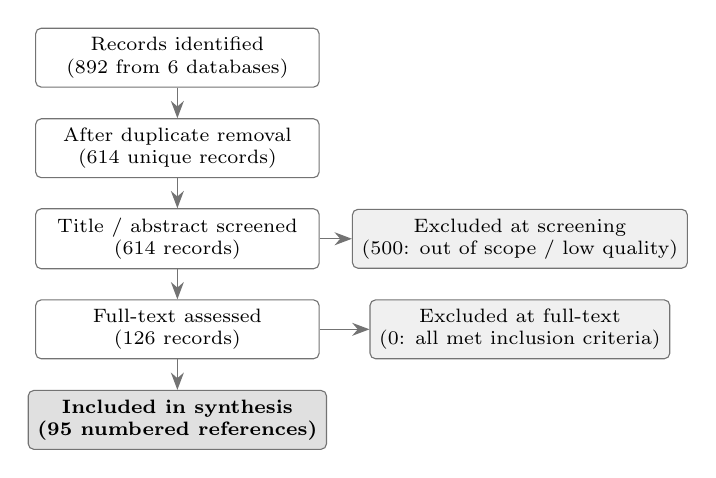
\begin{tikzpicture}[prisma/.style={draw=black!55, fill=white, rounded corners=2pt, minimum width=3.6cm, minimum height=0.72cm, align=center, font=\scriptsize}, prismaem/.style={prisma, fill=black!6, minimum width=3.0cm, minimum height=0.58cm}, arr/.style={-{Stealth[length=2.2mm]}, line width=0.45pt, draw=black!55}
]
  \node[prisma] (id) at (0,0) {Records identified\\(892 from 6 databases)};
  \node[prisma] (dedup) at (0,-1.15) {After duplicate removal\\(614 unique records)};
  \node[prisma] (screen) at (0,-2.3) {Title / abstract screened\\(614 records)};
  \node[prismaem] (excl1) at (4.35,-2.3) {Excluded at screening\\(500: out of scope / low quality)};
  \node[prisma] (full) at (0,-3.45) {Full-text assessed\\(126 records)};
  \node[prismaem] (excl2) at (4.35,-3.45) {Excluded at full-text\\(0: all met inclusion criteria)};
  \node[prisma, fill=black!12, font=\scriptsize\bfseries] (incl) at (0,-4.6)
    {Included in synthesis\\(95 numbered references)};
  \draw[arr] (id) -- (dedup);
  \draw[arr] (dedup) -- (screen);
  \draw[arr] (screen) -- (full);
  \draw[arr] (full) -- (incl);
  \draw[arr] (screen.east) -- (excl1.west);
  \draw[arr] (full.east) -- (excl2.west);
\end{tikzpicture}
\caption[PRISMA-style literature screening flow]{PRISMA-style literature screening flow}
\label{fig:prisma-flow}
\end{figure}

\section{Review of Existing Research}
\label{sec:review-existing}

We explain our literature review, and our findings from the papers and the work of the authors, in the subsections shown below.

\subsection{Decentralized Lending and DeFi Protocol Design}

For a big picture, Werner et al.~[1] show that DeFi lenders use flat pools with no bank-style tiers; we have found a gap that can be filled by introducing our project. According to Bastankhah et al.~[2], adaptive borrow rates work better than Aave-style curves for financial flows, which we introduced in our kinked-rate module. Dao et al.~[43] show how on-chain limits can get off-chain credit scores that in general are applied at our Local Bank level.

\subsection{Machine Learning, Explainable AI, and Extended AI Security}

For fraud detection, Palaiokrassas et al.~[3] engineer behavioral features that do a really good job in DeFi transaction fraud detection, not just hashes. We plan to use Random Forest in Phase~III that will further strengthen the fraud detection level with the mixture of hash functions that is built into the DeFi protocol. Moreover, for the situations when the fraud detection level is scarce, we will use Liu et al.~[6] Isolation Forest. We also studied a very in-depth comparison of SHAP versus LIME by Adom et al.~[4], which shows a significant advantage by using SHAP for loan detection; approvers in bank and authority level will see SHAP screening results before signing.

\subsection{Hierarchical Distribution, Cross-Tier Flows, and Group Lending}
\label{sec:lit-cross-tier}

Tan~[5] demonstrated how CBDC flows in bank-to-bank and bank-to-client financial transactions. We extended this idea in our project by showing tier-based reserve checks. For layered reserve contracts, \textit{Project Pine}~[79] has shown a prototype that is similar to our \texttt{InterBankLendingPool} and the syndicated-style loan flow. We also integrated the style of microcredit admin cost with smart contracts based on the study of Asaduzzaman et al.~[38]. The structure of \texttt{GroupLendingPool} function is the on-chain version, without claiming that we are trying to replace BRAC-style social microfinancing enforcement.

\subsection{Smart Contract Security and Layer~2 Scalability}

To improve the security system of the project, we are following Atzei et al.~[7], which lists the main Ethereum contract attacks. Since the tier-based system is very complex, many transactions on Cardona might be triggered. Gas prices can be cut to 30--50\% by transaction batching~[13], with further DeFi gas optimisation~[39].

\subsection{Monetary Policy, Tokenization, and Institutional Landscape}
\label{sec:lit-institutional}

Very large institutions like World Bank FundsChain~[27] and similar institutions show that development finance is already moving on-chain for auditability; we are further improving this by encoding rules, not just managing disbursement logs.

\subsection{Graph ML, Federated Learning, Regulation, and Identity Primitives}

We noticed the usability and rise of stablecoin and went further deep into it and try to explore how stablecoin pools for retail clients can be strengthened by using MiCA and the U.S.\ GENIUS Act~[61, 63]. For our project, soulbound tokens will be used that fit into our Credit Passport idea, which was extended by the idea of Buterin et al.~[55]. This introduces a secured identity on-chain, a portable reputation, without the fear of exposing personal data.

\subsection{Oracle-Mediated ML and Optional LLM Interfaces}
\label{sec:lit-llm}

Lastly, for an optional feature to our project, future studies can be made and features can be added to the system. Caldarelli~[76] describes how ML scores still have some issues that go beyond price oracles; we focus on this part and extend our commit-reveal or Chainlink path targets. We collected some reputable databases, and more to be added such as the BCCC fraud dataset~[71] that goes with our system. This section will be continued and extended after pre-thesis~2.

\begin{table}[H]
\centering
\footnotesize
\setlength{\tabcolsep}{3pt}
\renewcommand{\arraystretch}{1.08}
\caption[Literature review summary (Part 1 of 2)]{Literature review summary (Part 1 of 2)}
\label{tab:lit-summary}
\resizebox{\textwidth}{!}{%
\begin{tabular}{@{}>{\raggedright\arraybackslash}p{3.0cm}>{\raggedright\arraybackslash}p{2.6cm}>{\raggedright\arraybackslash}p{6.8cm}@{}}
\toprule
\tableheadcolor
\tableheadfont Author \& Focus & \tableheadfont Methodology & \tableheadfont What they found \& how we use it \\
\midrule
Palaiokrassas et al.\ (2024) [3] · DeFi fraud & XGBoost, NN on 54M+ txs & We plan to use behavioural features in Phase~II for Random Forest, as it lifted F1 to 0.76--0.85 \\
Adom et al.\ (2025) [4] · XAI lending & LIME / SHAP comparison & Approvers get a SHAP brief before signing, as it gives a clearer result than LIME on loan data \\
Tan (2023) [5] · CBDC hierarchy & Developing-nation model & CBDC backs the four-tier layout and works as a bank-to-user tier \\
Liu et al.\ (2008) [6] · Anomaly detection & Isolation Forest & Flags odd wallets without many labels; backup when fraud data is thin \\
Atzei et al.\ (2017) [7] · SC security & SoK of Ethereum attacks & Lists re-entrancy and access-control risks; guides OpenZeppelin guards \\
Werner et al.\ (2022) [1] · DeFi SoK & Survey of 12+ protocol types & Main gap CWB targets is DeFi lending having no bank hierarchy \\
Bastankhah et al.\ (2024) [2] · Adaptive lending & Dual fast/slow control & Dynamic rates support our kinked-rate modules as it beats static curves \\
Hartmann \& Hasan (2021) [32] · P2P lending & Smart-contract origination & Gas is cut in on-chain P2P, which is a minor input for loan-facing clients \\
Hasan et al.\ (2022) [33] · Federated fraud & FL on encrypted features & Lack of raw-data sharing features by banks leaves future cross-bank options \\
Wang et al.\ (2020) [34] · SC vulnerabilities & ML on bytecode & Common bytecode bugs spotting by ML helps provide extra security over manual audit \\
Liao et al.\ (2019) [35] · Audit automation & Classification + fuzzing & Workflow idea for Phase~V is inspired from ML prioritizing fuzzing speed \\
\bottomrule
\end{tabular}%
}
\end{table}

\begin{table}[H]
\centering
\footnotesize
\setlength{\tabcolsep}{3pt}
\renewcommand{\arraystretch}{1.08}
\caption[Literature review summary (Part 2 of 2)]{Literature review summary (Part 2 of 2)}
\label{tab:lit-summary-b}
\resizebox{\textwidth}{!}{%
\begin{tabular}{@{}>{\raggedright\arraybackslash}p{3.0cm}>{\raggedright\arraybackslash}p{2.6cm}>{\raggedright\arraybackslash}p{6.8cm}@{}}
\toprule
\tableheadcolor
\tableheadfont Author \& Focus & \tableheadfont Methodology & \tableheadfont What they found \& how we use it \\
\midrule
BIS et al.\ (2020) [37] · CBDC design & Retail distribution analysis & Standard CBDC two-tier is extended to four-tier with on-chain reserves \\
Kiff et al.\ (2020) [82] · CBDC models & IMF architecture survey & Matching National/Local roles; retail CBDC flow implemented through supervised banks \\
Bindseil (2020) [81] · CBDC rates & ECB tiered remuneration & Upward deposit spread idea inspired from tiered rates that protect bank intermediation \\
Dong et al.\ (2023) [80] · Supply-chain finance & Three-tier game model & Capital can move down a chain, parallel to World Bank $\to$ client allocation \\
Project Pine (2025) [79] · Hierarchical SCs & NY Fed / BIS prototype & IBLP and syndicated loans used on-chain layered reserve contracts prototype \\
CPMI/FSB [14, 21] · Cross-border settlement & Nostro/vostro cost analysis & Tiered on-chain flow is better than legacy settlement as it is slow and costly \\
World Bank (2025) [27] · Dev.\ finance blockchain & 13-project pilot & Programmable lending rules added with dev-banks system \\
Chen et al.\ (2024) [30] · Multi-chain lending & Cross-chain design & Scaling by splitting loads throughout chain is later option, not for Phase~I \\
Yang \& Cui (2023) [31] · Protocol evaluation & Quantitative risk metrics & Gives utilisation and liquidation benchmarks for health checks tier \\
Asaduzzaman et al.\ (2020) [38] · Smart micro-credit & Smart-contract MFI & Model for \texttt{GroupLendingPool} is smart contracts, which cuts the admin costs in Bangladesh \\
Wang et al.\ (2021) [13] · Tx batching & iBatch middleware & Per call saved 15--59\% in gas price by which we deploy on Cardona L2 \\
Kim \& Kim (2024) [39] · Gas optimisation & DeFi parameter tuning & $\sim$18\% gas cut on Ethereum pools helps our L2 deployment \\
Yuan (2024) [40] · SHAP credit default & RF, GBM + SHAP & Deploying on Cardona L2 as batching saved 30--50\% gas; SHAP is also used for our decline path \\
\bottomrule
\end{tabular}%
}
\end{table}

\begin{table}[H]
\centering
\footnotesize
\setlength{\tabcolsep}{3pt}
\resizebox{\textwidth}{!}{%
\begin{tabular}{@{}p{3.4cm}*{6}{>{\centering\arraybackslash}p{1.35cm}}@{}}
\toprule
\tableheadcolor
\tableheadfont Feature & \tableheadfont Aave & \tableheadfont Comp. & \tableheadfont Maker & \tableheadfont Maple & \tableheadfont Gfinch & \tableheadfont CWB \\
\midrule
Institutional hierarchy & \tmarkNo{} & \tmarkNo{} & \tmarkNo{} & \tmarkNo{} & \tmarkNo{} & \tmarkPlanned{} \\
\rowcolor{RowShade}
Cross-tier capital flow & \tmarkNo{} & \tmarkNo{} & \tmarkNo{} & \tmarkNo{} & \tmarkNo{} & \tmarkPartial{} \\
Same-tier interbank lending & \tmarkNo{} & \tmarkNo{} & \tmarkNo{} & \tmarkNo{} & \tmarkNo{} & \tmarkPartial{} \\
\rowcolor{RowShade}
Syndicated / co-lending & \tmarkNo{} & \tmarkNo{} & \tmarkNo{} & Part. & Part. & \tmarkPartial{} \\
Upward capital repatriation & \tmarkNo{} & \tmarkNo{} & \tmarkNo{} & \tmarkNo{} & \tmarkNo{} & \tmarkPartial{} \\
\rowcolor{RowShade}
Solidarity group lending & \tmarkNo{} & \tmarkNo{} & \tmarkNo{} & \tmarkNo{} & Part. & \tmarkPlanned{} \\
AI/ML fraud detection & \tmarkNo{} & \tmarkNo{} & \tmarkNo{} & Man. & Man. & \tmarkPlanned{} \\
\rowcolor{RowShade}
SHAP explainability & \tmarkNo{} & \tmarkNo{} & \tmarkNo{} & \tmarkNo{} & \tmarkNo{} & \tmarkPlanned{} \\
ZKP KYC compliance & \tmarkNo{} & \tmarkNo{} & \tmarkNo{} & \tmarkNo{} & \tmarkNo{} & \tmarkPlanned{} \\
\rowcolor{RowShade}
Kinked interest rate curve & \tmarkDone{} & \tmarkDone{} & Gov. & \tmarkDone{} & \tmarkNo{} & \tmarkPartial{} \\
Role-based access control & Part. & Part. & Gov. & \tmarkDone{} & Part. & \tmarkPlanned{} \\
\rowcolor{RowShade}
Institutional / L2 focus & \tmarkNo{} & \tmarkNo{} & \tmarkNo{} & \tmarkDone{} & Part. & \tmarkPlanned{} \\
TVL / Status (2026) & \$26B & \$1.4B & \$10B & \$2.6B & \$680M & Planning \\
\bottomrule
\end{tabular}%
}
\caption[Protocol comparison on eleven architectural dimensions]{Protocol comparison on eleven architectural dimensions}
\label{tab:protocol-comparison}
\label{sec:comparative-protocol}
\end{table}

\section{Summary of Key Findings}
\label{sec:lit-key-findings}

Four points stand out after reviewing and Table~\ref{tab:protocol-comparison}:

\begin{itemize}[noitemsep]
\item \textbf{Flat DeFi vs.\ tiers.} Large pool lenders~[1, 8] have no hierarchical bank currently, and it opens a door to explore how a hierarchical system would behave with DeFi. CBDC and Project Pine work~[5, 79] prove that nobody combines a four reserve-enforced tier with group lending and cross-tier financial flows and an ML oracle in a singular architecture.
\item \textbf{ML and security.} ML and security layers combined with behavioural fraud features and SHAP~[3, 4, 6] further extend the usability, feasibility, and adaptability of our project. Based on these literature reviews, we further improve our Phase~III pipeline; contract attack catalogues~[7] and L2 gas batching~[13, 39] justify OpenZeppelin guards to be added to our project.
\item \textbf{Groups and institutions.} We explored smart-contract microcredit in Bangladesh~[38] and World Bank on-chain pilots~[27] that gave us the idea and improved the implementation of \texttt{GroupLendingPool} function and institutional lending system.
\item \textbf{Regulation.} For regulation improvement and securities, MiCA and GENIUS~[61, 63] are accepted by stablecoin-first pools. Soulbound credit tokens~[55] fit the Credit Passport without putting KYC on-chain.
\end{itemize}

%% CHAPTER 3 (compressed): architecture essentials only
\chapter{System Architecture and Design}
\label{ch:architecture-compressed}

\section{Prototype Scope and Stack}
\label{sec:prototype-scope}

\begin{table}[H]
\centering
\caption[Prototype scope (summary)]{Prototype scope (summary)}
\label{tab:prototype-scope}
\footnotesize
\begin{tabular}{@{}p{7.2cm}>{\raggedleft\arraybackslash}p{5.5cm}@{}}
\toprule
\tableheadcolor
\tableheadfont Feature & \tableheadfont Status \\
\midrule
Four-tier RBAC (World / National / Local / Client) & Specified (Phase~I) \\
Loan lifecycle + installments & Specified / Phase~II \\
SavingsVault, GroupLendingPool, IBLP & Specified / Phase~II \\
RF + IF + SHAP oracle pipeline & Planned (Phase~III) \\
ZKP KYC, testnet deploy, Foundry sim & Planned (Phase~IV) \\
Optional MCP agent (17 tools) & Optional (Phase~III--IV) \\
\bottomrule
\end{tabular}
\end{table}

\section{System Architecture}
\label{sec:high-level-arch}
\label{sec:oracle-architecture}
\label{sec:ml-explainability}
\label{sec:aiml-support}
\label{sec:data-model-compressed}
\label{sec:multi-entity}
\label{sec:over-indebt}
\label{sec:interbank-pool}
\label{sec:bridge}
\label{sec:kinked-rate}
\label{sec:upward-flow}
\label{sec:credit-passport}
\label{sec:identity}

\begin{figure}[H]
\centering
\OnePageDiagram{cwb_architecture.pdf}
\caption[CWB system architecture]{CWB system architecture — contracts, oracle/ML integration, data partitioning, and cross-tier operations}
\label{fig:cwb-architecture}
\end{figure}

\section{Architecture Diagrams (Full Set)}
\label{sec:architecture-figures}

\begin{figure}[H]
\centering
\BalancedDiagram{fig-three-layer-arch.pdf}
\caption[Four-layer application architecture]{Four-layer application architecture}
\label{fig:three-layer-arch}
\end{figure}

\begin{figure}[H]
\centering
\BalancedDiagram{fig-component-architecture.pdf}
\caption[Component diagram (planning phase)]{Component diagram (planning phase)}
\label{fig:component-diagram}
\end{figure}

\begin{figure}[H]
\centering
\BalancedDiagram{fig-blockchain-stack.pdf}
\caption[Layered blockchain and application stack]{Layered blockchain and application stack}
\label{fig:blockchain-stack}
\end{figure}

\begin{figure}[H]
\centering
\BalancedDiagram{fig-oracle-architecture.pdf}
\caption[Chainlink oracle architecture]{Chainlink oracle architecture}
\label{fig:oracle-architecture}
\end{figure}

\begin{figure}[H]
\centering
\BalancedDiagram{fig-erd-core.pdf}
\caption[Core system entity graph]{Core system entity graph}
\label{fig:core-system-graph}
\end{figure}

\begin{figure}[H]
\centering
\BalancedDiagram{fig-eer-model.pdf}
\caption[Enhanced EER model]{Enhanced EER model}
\label{fig:eer}
\end{figure}

\begin{figure}[H]
\centering
\BalancedDiagram{fig-erd-extended.pdf}
\caption[Extended ERD entities]{Extended ERD entities}
\label{fig:erd-extended}
\end{figure}

\begin{figure}[H]
\centering
\BalancedDiagram{fig-data-partitioning.pdf}
\caption[On-chain versus off-chain data partitioning]{On-chain versus off-chain data partitioning}
\label{fig:data-partitioning}
\end{figure}

\begin{figure}[H]
\centering
\BalancedDiagram{fig-compliance-identity.pdf}
\caption[Compliance and identity stack]{Compliance and identity stack}
\label{fig:compliance-identity}
\end{figure}

\begin{figure}[H]
\centering
\ThesisIncludeGraphics[width=0.9\linewidth, keepaspectratio]{Ch3_actor-permission-matrix.pdf}
\caption[Actor permission matrix (primary actions)]{Actor permission matrix (primary actions)}
\label{fig:permission-matrix}
\end{figure}

\begin{figure}[H]
\centering
\BalancedDiagram{fig-tier-model.pdf}
\caption[Client limits and bank-level syndication]{Client limits and bank-level syndication}
\label{fig:tier-model}
\end{figure}

\begin{figure}[H]
\centering
\BalancedDiagram{fig-five-stage-funnel.pdf}
\caption[Five-stage retail onboarding funnel]{Five-stage retail onboarding funnel}
\label{fig:five-stage-funnel}
\end{figure}

\begin{figure}[H]
\centering
\BalancedDiagram{fig-agent-six-step-pipeline.pdf}
\caption[Optional AI agent add-on (Phase III--IV, excluded from MVT)]{Optional AI agent add-on (Phase III--IV, excluded from MVT)}
\label{fig:agent-six-step-pipeline}
\end{figure}

\begin{figure}[H]
\centering
\HalfWidthDiagram{fig-liquidation-engine.pdf}
\caption[LiquidationEngine tier models and lifecycle]{LiquidationEngine tier models and lifecycle}
\label{fig:liquidation-engine}
\end{figure}

\begin{figure}[H]
\centering
\ThesisIncludeGraphics[width=0.9\linewidth, keepaspectratio]{fig-savings-vault.pdf}
\caption[SavingsVault and FixedDeposit closed loop]{SavingsVault and FixedDeposit closed loop}
\label{fig:savings-vault}
\end{figure}

\begin{figure}[H]
\centering
\HalfWidthDiagram{fig-credit-passport.pdf}
\caption[On-chain Credit Passport SBT lifecycle]{On-chain Credit Passport SBT lifecycle}
\label{fig:credit-passport}
\end{figure}

\begin{figure}[H]
\centering
\BalancedDiagram{fig-ccip-bridge.pdf}
\caption[Chainlink CCIP cross-chain hierarchy invariant]{Chainlink CCIP cross-chain hierarchy invariant}
\label{fig:ccip-bridge}
\end{figure}

\begin{figure}[H]
\centering
\BalancedDiagram{Ch3_multi-entity-cross-tier-operations.pdf}
\caption[Multi-entity and cross-tier capital operations]{Multi-entity and cross-tier capital operations}
\label{fig:multi-entity-ops}
\end{figure}

\begin{figure}[H]
\centering
\BalancedDiagram[width=0.98\linewidth]{Ch3_use-case-nine-actor-taxonomy.pdf}
\caption[Use-case diagram (nine-actor taxonomy)]{Use-case diagram (nine-actor taxonomy)}
\label{fig:usecase}
\end{figure}

\begin{figure}[H]
\centering
\ActivityDiagram{fig-activity-lending.pdf}
\caption[USDC loan lifecycle activity flow]{USDC loan lifecycle activity flow}
\label{fig:act-lending}
\label{fig:act-loan}\label{fig:act-hierarchy}
\end{figure}

\begin{figure}[H]
\centering
\ActivityDiagram{fig-activity-onboarding-id.pdf}
\caption[Retail onboarding and identity activity flow]{Retail onboarding and identity activity flow}
\label{fig:act-onboarding}
\label{fig:act-income}\label{fig:act-profile}
\end{figure}

\begin{figure}[H]
\centering
\ActivityDiagram{fig-activity-aux.pdf}
\caption[Client banking session activity flow]{Client banking session activity flow}
\label{fig:act-aux}
\label{fig:act-chat}\label{fig:act-aichatbot}\label{fig:act-market}
\end{figure}

\begin{figure}[H]
\centering
\BalancedDiagram{Ch3_data-flow-diagrams.pdf}
\caption[Data-flow diagrams]{Data-flow diagrams}
\label{fig:dfd-suite}
\label{fig:dfd-context}\label{fig:dfd-level1a}\label{fig:dfd-level1b}
\end{figure}

\begin{figure}[H]
\centering
\BalancedDiagram{fig-seq-loan-flow.pdf}
\caption[Loan approval sequence diagram]{Loan approval sequence diagram}
\label{fig:seq-loan-flow}
\label{fig:seq-loan}\label{fig:seq-reject}
\end{figure}

\begin{figure}[H]
\centering
\BalancedDiagram{fig-seq-installment-income.pdf}
\caption[Sequence diagrams]{Sequence diagrams}
\label{fig:seq-installment-income}
\label{fig:seq-installment}\label{fig:seq-income}
\end{figure}

\begin{figure}[H]
\centering
\BalancedDiagram{fig-seq-banking-data.pdf}
\caption[Sequence diagrams]{Sequence diagrams}
\label{fig:seq-banking-data}
\label{fig:seq-hierarchy}\label{fig:seq-marketdata}\label{fig:seq-borrowlimit}
\end{figure}

\begin{figure}[H]
\centering
\BalancedDiagram{fig-seq-chat-chatbot.pdf}
\caption[Sequence diagrams]{Sequence diagrams}
\label{fig:seq-chat-bot}
\label{fig:seq-chat}\label{fig:seq-aichatbot}
\end{figure}

\begin{figure}[H]
\centering
\BalancedDiagram{fig-hierarchical-banking.pdf}
\caption[Four-tier hierarchical capital flow]{Four-tier hierarchical capital flow}
\label{fig:four-tier}
\end{figure}

\begin{figure}[H]
\centering
\BalancedDiagram{fig-governance-dual-path.pdf}
\caption[Governance dual-path]{Governance dual-path}
\label{fig:governance-dual-path}
\end{figure}

\begin{figure}[H]
\centering
\BalancedDiagram{fig-sar-aml-workflow.pdf}
\caption[SAR and AML compliance workflow]{SAR and AML compliance workflow}
\label{fig:sar-aml-workflow}
\end{figure}

\begin{figure}[H]
\centering
\BalancedDiagram{fig-defense-in-depth.pdf}
\caption[Five-layer defense-in-depth security architecture]{Five-layer defense-in-depth security architecture}
\label{fig:defense-in-depth}
\label{sec:defense-in-depth}
\end{figure}

\begin{figure}[H]
\centering
\BalancedDiagram{fig-security-controls.pdf}
\caption[Smart-contract security controls]{Smart-contract security controls}
\label{fig:security-controls}
\end{figure}
%% CHAPTER 4 (compressed): methodology summary
\chapter{Methodology}
\label{ch:methodology-compressed}

Lightweight \textbf{Agile/Scrum} across four implementation phases. \textbf{Core thesis} = on-chain banking + oracle ML; conversational agent is optional (Could-have).

\section{MVT Checklist and Phase Plan}
\label{sec:mvt-checklist}

Graded pass line: (C1) four-tier contracts on testnet; (C2) \texttt{GroupLendingPool} spec + PoC; (C3) RF/IF/SHAP + Authority Brief after pre-thesis~2. Pre-thesis~1 delivers specification only---no trained models or live deploy.

\begin{table}[H]
\centering
\caption[Four-phase implementation summary]{Four-phase implementation summary}
\label{tab:phase-summary}
\begin{tabular}{p{1.4cm}p{3.8cm}p{1.6cm}p{6.5cm}}
\toprule
\tableheadcolor
\textbf{Phase} & \textbf{Focus} & \textbf{Weeks} & \textbf{Key deliverables} \\
\midrule
I & Foundation & 1--4 & Contract hierarchy, DB schema, React shell \\
II & Core banking & 5--9 & Loan E2E, savings, group pool, automation \\
III & ML + oracle & 10--13 & Chainlink Functions, Authority Brief, dashboard \\
IV & Verification & 14--16 & Foundry sim, Certora stretch, testnet manifest \\
\bottomrule
\end{tabular}
\end{table}

\begin{table}[H]
\centering
\caption[Core vs.\ optional capabilities]{Core vs.\ optional capabilities}
\label{tab:capability-priority}
\begin{tabular}{p{3.2cm}p{2.2cm}p{7.8cm}}
\toprule
\tableheadcolor
\textbf{Capability} & \textbf{Priority} & \textbf{Phase / interface} \\
\midrule
Four-tier smart contracts & Must (I--II) & React + wallet; Foundry tests \\
On-chain loan lifecycle & Must (II) & \texttt{LoanController} state machine \\
Chainlink Functions oracle & Must (III) & FastAPI $\to$ DON $\to$ on-chain score \\
RF + IF + SHAP & Must (III) & Authority Brief; audit log \\
MCP conversational agent & Could (III--IV) & Alternate API path only \\
\bottomrule
\end{tabular}
\end{table}

\section{Design Decisions}
\label{sec:design-decisions}
\label{sec:gnn-extension}
\label{sec:fl-fraud}
\label{sec:ml-workload}

\begin{table}[H]
\centering
\caption[Design decisions (selected)]{Design decisions (selected)}
\label{tab:design-decisions}
\footnotesize
\begin{tabular}{p{2.8cm}p{2.6cm}p{2.6cm}p{4.5cm}}
\toprule
\tableheadcolor
\textbf{Area} & \textbf{Choice} & \textbf{Alternative} & \textbf{Criterion} \\
\midrule
Network & Polygon zkEVM Cardona & Amoy PoS & ZK validity proofs, low gas \\
Contracts & Solidity EVM & Solana & Tooling, testnet cost \\
Fraud ML & Random Forest + IF & XGBoost & SHAP compatibility \\
Oracle & Chainlink Functions & Commit-reveal only & Decentralised trust \\
Database & PostgreSQL & SQLite & 3NF, async API \\
\bottomrule
\end{tabular}
\end{table}


\section{Methodology Diagrams (Full Set)}
\label{sec:methodology-figures}
\label{sec:llm-eval}
\label{sec:future-retail-payments}

\begin{figure}[H]
\centering
\BalancedDiagram{fig-agile-process.pdf}
\caption[Agile / Scrum development process]{Agile / Scrum development process}
\label{fig:agile-process}
\end{figure}

\begin{figure}[H]
\centering
\BalancedDiagram{fig-aiml-pipeline.pdf}
\caption[AI/ML pipeline wiring]{AI/ML pipeline wiring}
\label{fig:aiml-pipeline}
\end{figure}

\begin{figure}[H]
\centering
\small
\begin{minipage}[t]{0.48\linewidth}
\centering
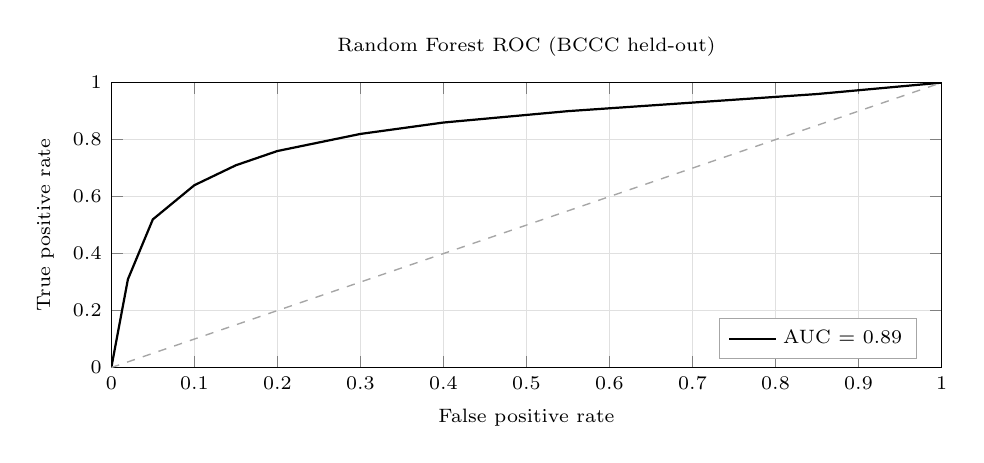
\begin{tikzpicture}
\begin{axis}[
 width=\linewidth,
 height=5.2cm,
 xlabel={False positive rate},
 ylabel={True positive rate},
 xmin=0, xmax=1,
 ymin=0, ymax=1,
 grid=both,
 grid style={black!12},
 tick label style={font=\scriptsize},
 label style={font=\scriptsize},
 title={\scriptsize Random Forest ROC (BCCC held-out)},
 title style={font=\scriptsize},
 legend style={font=\scriptsize, at={(0.97,0.03)}, anchor=south east, draw=black!35, fill=white},
]
\addplot[black, line width=0.8pt, mark=none]
 coordinates {
 (0,0) (0.02,0.31) (0.05,0.52) (0.10,0.64) (0.15,0.71)
 (0.20,0.76) (0.30,0.82) (0.40,0.86) (0.55,0.90) (0.70,0.93)
 (0.85,0.96) (1,1)
 };
\addlegendentry{AUC = 0.89}
\addplot[black!35, dashed, line width=0.5pt] coordinates {(0,0) (1,1)};
\end{axis}
\end{tikzpicture}

\vspace{4pt}
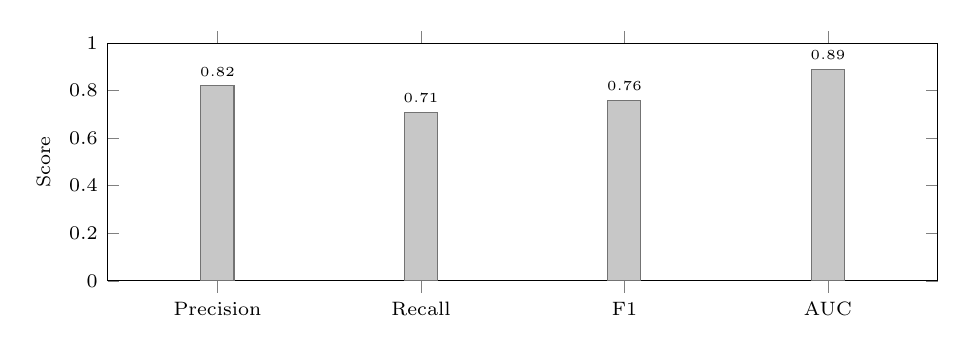
\begin{tikzpicture}
\begin{axis}[
 width=\linewidth,
 height=4.6cm,
 ybar,
 bar width=0.42cm,
 symbolic x coords={Precision, Recall, F1, AUC},
 xtick=data,
 ymin=0, ymax=1,
 ylabel={Score},
 tick label style={font=\scriptsize},
 label style={font=\scriptsize},
 nodes near coords={\pgfmathprintnumber[fixed, precision=2]{\pgfplotspointmeta}},
 every node near coord/.append style={font=\tiny},
 enlarge x limits=0.18,
]
\addplot[fill=black!22, draw=black!55] coordinates {
 (Precision, 0.82) (Recall, 0.71) (F1, 0.76) (AUC, 0.89)
};
\end{axis}
\end{tikzpicture}
\end{minipage}\hfill
\begin{minipage}[t]{0.48\linewidth}
\centering
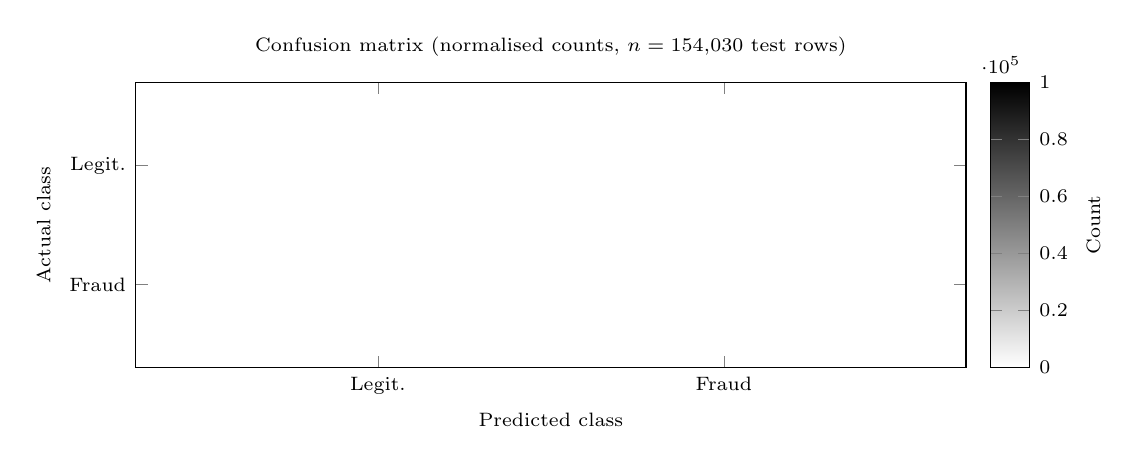
\begin{tikzpicture}
\begin{axis}[width=\linewidth, height=5.2cm, xlabel={Predicted class}, ylabel={Actual class}, xtick={0, 1}, ytick={0, 1}, xticklabels={Legit., Fraud}, yticklabels={Legit., Fraud}, tick label style={font=\scriptsize}, label style={font=\scriptsize}, title={\scriptsize Confusion matrix (normalised counts, $n=154{, }030$ test rows)}, title style={font=\scriptsize}, colorbar, colormap={greyscale}{color(0cm)=(white); color(1cm)=(black!)}, point meta min=0, point meta max=100000, colorbar style={font=\scriptsize, ylabel={Count}}, ]
\addplot[matrix plot, mesh/cols=2, mesh/rows=2, shader=flat corner, ] table[meta=z] {
 x y z
 0 0 98420
 1 0 1180
 0 1 820
 1 1 610
};
\end{axis}
\end{tikzpicture}

\vspace{4pt}
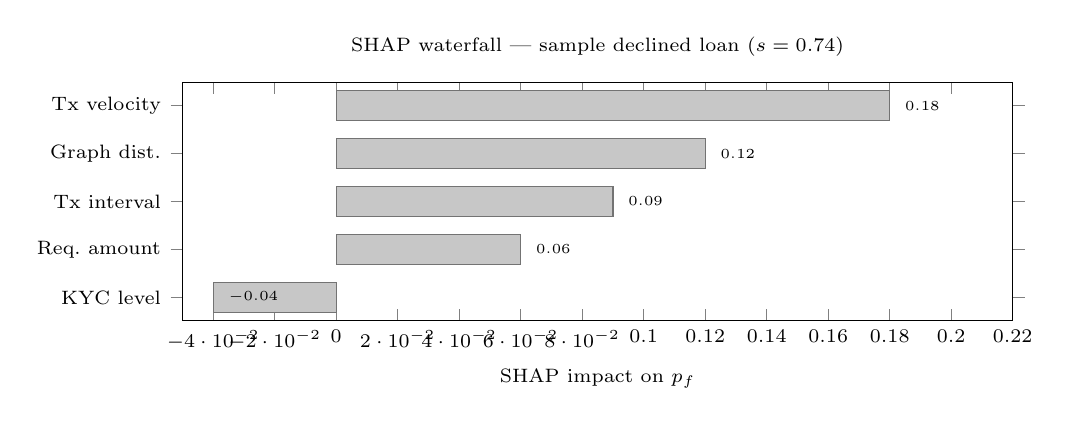
\begin{tikzpicture}
\begin{axis}[
 width=\linewidth,
 height=4.6cm,
 xbar,
 bar width=0.38cm,
 xmin=-0.05, xmax=0.22,
 symbolic y coords={%
 KYC level, Req.\ amount, Tx interval, Graph dist., Tx velocity%
 },
 ytick=data,
 xlabel={SHAP impact on $p_f$},
 tick label style={font=\scriptsize},
 label style={font=\scriptsize},
 title={\scriptsize SHAP waterfall --- sample declined loan ($s=0.74$)},
 title style={font=\scriptsize},
 nodes near coords={\pgfmathprintnumber[fixed, precision=2]{\pgfplotspointmeta}},
 every node near coord/.append style={font=\tiny, anchor=west, xshift=2pt},
 enlarge y limits=0.12,
]
\addplot[fill=black!22, draw=black!55] coordinates {
 (0.18,Tx velocity) (0.12,Graph dist.) (0.09,Tx interval)
 (0.06,Req.\ amount) (-0.04,KYC level)
};
\end{axis}
\end{tikzpicture}
\end{minipage}
\caption[Planned ML evaluation layout (post pre-thesis 2)]{Planned ML evaluation layout (post pre-thesis 2)}
\label{fig:ml-eval}
\end{figure}

\begin{figure}[H]
\centering
\BalancedDiagram{fig-ml-explainability.pdf}
\caption[Explainability and anomaly-detection flow]{Explainability and anomaly-detection flow}
\label{fig:ml-explainability}
\end{figure}

\begin{figure}[H]
\centering
\ActivityDiagram{fig-realtime-dashboard.pdf}
\caption[Real-time dashboard and runtime monitoring pipeline]{Real-time dashboard and runtime monitoring pipeline}
\label{fig:realtime-dashboard}
\end{figure}

\begin{figure}[H]
\centering
\BalancedDiagram{Ch4_loan-lifecycle-state-machine.pdf}
\caption[Transaction state machine of the loan lifecycle]{Transaction state machine of the loan lifecycle}
\label{fig:tx-state-machine}
\end{figure}

\begin{figure}[H]
\centering
\ThesisIncludeGraphics[width=\linewidth, height=\textheight, keepaspectratio]{Ch4_four-phase-roadmap-sdlc.pdf}
\caption[Four-phase roadmap with SDLC mapping and progress]{Four-phase roadmap with SDLC mapping and progress}
\label{fig:phase-roadmap}
\end{figure}

\begin{figure}[H]
\centering
\ThesisIncludeGraphics[width=0.6\linewidth, height=0.432\textheight, keepaspectratio]{fig-phase-effort-bar.pdf}
\caption[Development effort by implementation phase]{Development effort by implementation phase}
\label{fig:phase-effort}
\end{figure}

\begin{figure}[H]
\centering
\ThesisIncludeGraphics[width=0.75\linewidth, height=0.54\textheight, keepaspectratio]{fig-optional-agent-addon.pdf}
\caption[Optional conversational agent add-on]{Optional conversational agent add-on}
\label{fig:optional-agent-addon}
\end{figure}

\begin{figure}[H]
\centering
\ActivityDiagram{Ch4_dev-verification-toolchain.pdf}
\caption[Planned development and verification toolchain]{Planned development and verification toolchain}
\label{fig:dev-toolchain}
\end{figure}

\begin{figure}[H]
\centering
\BalancedDiagram{Ch4_design-decisions-alternatives.pdf}
\caption[Key design decisions and alternatives considered]{Key design decisions and alternatives considered}
\label{fig:design-decisions}
\end{figure}
%% CHAPTER 5 (compressed)
\chapter{Evaluation and Discussion}
\label{ch:evaluation-compressed}

\section{Performance Evaluation}
\label{sec:performance-eval}
\label{sec:cost-model}
\label{sec:gas-cost}
\label{sec:eval-method}

Our pre-thesis~1 shows specifications and plans and creates checkboxes, not any kind of live benchmarks, since the project has not been deployed or tested yet. Project influential elements and financial feasibility are further elaborated in Section~\ref{sec:feasibility}. Our planned RQ-level evaluation will be executed after pre-thesis~2. Our plan is for projected gas per loan to stay below interest achieved on L2; the result of default stress is given in Table~\ref{tab:default-scenarios}.

\section{Analysis of Design Solutions}
\label{sec:design-solutions-ch5}

Our choices of technology stack were chosen based on ecosystem maturity, as per our goal to create a system with zero-cost prototype constraints and more transparent auditability (visible in Table~\ref{tab:design-decisions}, Section~\ref{sec:design-decisions}). The chosen stack for off-chain pairs EVM Solidity on PostgreSQL + FastAPI, zkEVM for L2 execution, and to connect to on-chain we use Chainlink Functions attached with ML scores. The optional conversational MCP agent and EIP-7702 session keys remain Phase~III--IV extensions outside the MVT.

\section{Final Design Adjustment}
\label{sec:final-design-adjustment}

The final pre-thesis~1 outlook locks in four adjustments before implementation. These are stablecoins, which is the first retail lending path and is used to avoid ETH liability volatility (USDC/USDT, Section~\ref{sec:stablecoin-first}). After that, L2 deployment for micro-loan gas economics. The third one is ML as decision support only, meaning human approvers and on-chain gates, no auto-disbursement. Last but not least is MVT scope. It is limited to the three-tier lending core, database schema, and dashboard; syndicated modules, full regulatory filing, and the conversational agent are deferred.

\section{Feasibility Analysis}
\label{sec:feasibility}

\subsection{Technical Feasibility}

Each layer is specified against mature tooling; nothing requires bespoke infrastructure beyond standard testnets and open-source stacks (Table~\ref{tab:tech-feasibility}).

\begin{table}[H]
\centering
\caption[Technical feasibility assessment]{Technical feasibility assessment}
\label{tab:tech-feasibility}
\begin{tabular}{p{3cm}p{3cm}p{7.5cm}}
\toprule
\tableheadcolor
\textbf{Component} & \textbf{Assessment} & \textbf{Evidence} \\
\midrule
Smart contracts & Feasible (specified) & Solidity; Hardhat; OpenZeppelin; Phases~I--II \\
Frontend DApp & Feasible (specified) & React~18 + Wagmi/RainbowKit \\
Blockchain deployment & Feasible (planned) & Polygon zkEVM Cardona + Sepolia \\
AI/ML integration & Feasible with constraints & RF + IF + SHAP; Chainlink Functions Phase~III \\
Optional agent & Feasible (deferred) & MCP + Qwen3-8B; Phase~III--IV; outside MVT \\
Database backend & Feasible & PostgreSQL 20-entity schema (3NF); FastAPI \\
\bottomrule
\end{tabular}
\end{table}

\vspace{2pt}

\subsection{Economic Feasibility}

\begin{table}[H]
\centering
\caption[Economic feasibility --- zero-cost prototype]{Economic feasibility --- zero-cost prototype}
\label{tab:economic-feasibility}
\begin{tabular}{p{4cm}p{2.5cm}p{7cm}}
\toprule
\tableheadcolor
\textbf{Cost Category} & \textbf{Estimate} & \textbf{Notes} \\
\midrule
Blockchain deployment & \$0 & Public testnets \\
Frontend / backend hosting & \$0 & Vercel / Render free tiers or localhost \\
AI/ML training & \$0 & Local machine or Colab free tier \\
Development tools & \$0 & Hardhat, VS Code, Git (open-source) \\
\textbf{Total prototype} & \textbf{\$0} & Pilot ops $\approx$\$500--\$2{,}000/month at scale \\
\bottomrule
\end{tabular}
\end{table}

\vspace{2pt}

\subsection{Risk Feasibility}

Main delivery risks and mitigations are summarised in Table~\ref{tab:risk-taxonomy}; smart-contract and regulatory items dominate severity.

\begin{table}[H]
\centering
\caption[Risk taxonomy and mitigation]{Risk taxonomy and mitigation}
\label{tab:risk-taxonomy}
\begin{tabular}{p{3cm}p{4cm}p{1.5cm}p{5cm}}
\toprule
\tableheadcolor
\textbf{Risk Category} & \textbf{Description} & \textbf{Severity} & \textbf{Mitigation} \\
\midrule
Partner non-cooperation & Key partners decline to join & Medium & Testnet pilots; open-source replication \\
Smart contract vulnerability & Logic exploit & High & OpenZeppelin; audits; pause mechanism \\
Regulatory adversity & Jurisdiction blocks retail crypto & Medium & Testnet-only prototype; sandbox path \\
AI/ML model degradation & Fraud model drift & Low & Retraining; human-in-the-loop; SHAP review \\
\bottomrule
\end{tabular}
\end{table}

\vspace{2pt}

\subsection{Regulatory Feasibility}
\label{sec:mica-compliance}

The CWB platform uses basic compliance measures for retail stablecoin lending like MiCA, GENIUS Act, and EU AI Act, using authorized stablecoin and keeping PII off-chain (Table~\ref{tab:mica-mapping}). But for future work, full conformity files and national licensing are kept. This thesis only focuses on testnet.

\begin{table}[H]
\centering
\caption[Regulatory design controls (selected)]{Regulatory design controls (selected)}
\label{tab:mica-mapping}
\begin{tabular}{p{3.2cm}p{4.6cm}p{5.8cm}}
\toprule
\tableheadcolor
\textbf{Statute / Article} & \textbf{Requirement} & \textbf{CWB Control} \\
\midrule
MiCA Art.~16 & Authorised EMT issuer & Uses USDC/USDT; does not issue \\
MiCA Art.~36 & 1{:}1 reserve backing & Issuer attestations before pool acceptance \\
EU AI Act (credit scoring) & High-risk AI from Aug.~2026~ & Human approver gate; SHAP + audit log \\
GDPR Art.~17 & Right to erasure & PII off-chain only; hashes on-chain \\
\bottomrule
\end{tabular}
\end{table}

\section{Statistical Analysis}
\label{sec:statistical-analysis}
\label{sec:interest-rates}

Based on planning assumption rather than platform data, the table below presents spread revenue, ETH-price sensitivity, and default stress at deployment scale. As shown in Figure~\ref{fig:apr-spread}, the interest structure follows the lending hierarchy of 3\%, 5\%, and 8\%.

\begin{table}[H]
\centering
\caption[Revenue projection assumptions]{Revenue projection assumptions}
\label{tab:revenue-assumptions}
\begin{tabular}{p{6cm}p{7.5cm}}
\toprule
\tableheadcolor
\textbf{Parameter} & \textbf{Value} \\
\midrule
Reference ETH price & \$2{,}500 (planning mid-point, Feb 2026) \\
World Bank $\to$ National Bank & 3\% APR \\
National Bank $\to$ Local Bank & 5\% APR \\
Local Bank $\to$ Client & 8\% APR \\
Average loan term & 12 months \\
Default rate provision (base) & 8\% \\
Origination fee & 0.25\% per disbursement \\
\bottomrule
\end{tabular}
\end{table}

\vspace{2pt}

\begin{table}[H]
\centering
\caption[ETH-price sensitivity of spread revenue]{ETH-price sensitivity of spread revenue}
\begin{tabular}{@{}lccc@{}}
\toprule
\tableheadcolor
\tableheadfont ETH Price & \tableheadfont Loan Base & \tableheadfont Spread Revenue & \tableheadfont Incl.\ Fees (est.) \\
\midrule
\$2{,}000 & \$1.376B & \$110.1M & \$120--128M \\
\rowcolor{RowShade}
\$2{,}500 (base) & \$1.720B & \$137.6M & \$150--159M \\
\$3{,}000 & \$2.064B & \$165.1M & \$180--191M \\
\bottomrule
\end{tabular}
\end{table}

\vspace{2pt}

\begin{table}[H]
\centering
\caption[Default-rate sensitivity]{Default-rate sensitivity}
\label{tab:default-scenarios}
\begin{tabular}{@{}lccp{4.8cm}@{}}
\toprule
\tableheadcolor
\tableheadfont Scenario & \tableheadfont Default rate & \tableheadfont Annual loss & \tableheadfont Basis \\
\midrule
Optimistic & 3.7\% & \$7.4M & Mature MFI benchmarks~ \\
\rowcolor{RowShade}
Base case & 8\% & \$16M & New platform, limited history \\
Stress & 15\% & \$30M & Thin credit history, volatile collateral \\
\bottomrule
\end{tabular}
\end{table}

\begin{figure}[H]
\centering
\HalfWidthDiagram{fig-revenue-by-tier.pdf}
\caption[Annual revenue projection (10-year maturity)]{Annual revenue projection (10-year maturity)}
\label{fig:revenue-by-tier}
\end{figure}

\begin{figure}[H]
\centering
\HalfWidthDiagram{fig-apr-spread.pdf}
\caption[Hierarchical interest-rate spread (APR)]{Hierarchical interest-rate spread (APR)}
\label{fig:apr-spread}
\end{figure}

\section{Comparisons and Relationships}
\label{sec:comparisons-relationships}

\begin{table}[H]
\centering
\caption[Market segments with supporting data]{Market segments with supporting data}
\label{tab:market-sizing-ch5}
\begin{tabular}{p{3.5cm}p{6.5cm}p{3cm}}
\toprule
\tableheadcolor
\textbf{Segment} & \textbf{Description} & \textbf{Estimated Scale} \\
\midrule
TAM & Global DeFi lending; remittances; MSME gap~[8, 11, 16] & \$55B -- 5T+ \\
SAM & Institutional hierarchical lending; emerging-market credit & \$5B -- 15B \\
SOM & Testnet pilots; sandbox partnerships & \$50 -- 200M \\
\bottomrule
\end{tabular}
\end{table}

\vspace{2pt}

\begin{table}[H]
\centering
\caption[Target customer segment profile]{Target customer segment profile}
\label{tab:customer-segment-ch5}
\begin{tabular}{p{3.5cm}p{10cm}}
\toprule
\tableheadcolor
\textbf{Characteristic} & \textbf{Description} \\
\midrule
Primary users & Tier~1--3 bank operators; Tier~4 retail via Local Banks \\
Loan range & Micro/SME at Local Bank tier; larger exposures via syndication \\
Key pain points & Opaque reserves; flat DeFi pools; weak explainability in on-chain lending \\
\bottomrule
\end{tabular}
\end{table}

\vspace{2pt}

\begin{table}[H]
\centering
\caption[Partner categories and roles]{Partner categories and roles}
\label{tab:partner-categories-ch5}
\begin{tabular}{p{3.5cm}p{4.5cm}p{5.5cm}}
\toprule
\tableheadcolor
\textbf{Partner Category} & \textbf{Role} & \textbf{Incentive} \\
\midrule
Financial regulators & Sandbox oversight & On-chain audit trails \\
Banking institutions & National/Local Bank nodes & Reserve access; lower settlement friction \\
Oracle providers & Chainlink DON, indexing & Unified oracle stack \\
Academic partners & ML / formal-verification review & Datasets; co-publication \\
\bottomrule
\end{tabular}
\end{table}

\section{Discussion}
\label{sec:ch5-discussion}
\label{sec:research-limitations}
\label{sec:bangladesh-reg}

This pre-thesis only shows architecture and evaluation plans. The deployment result, trained model and formal proof will be evaluated on pre-thesis~2. Five key limitations are:

\begin{itemize}[noitemsep]
\item \textbf{Novelty is compound, not absolute:} this thesis uniquely represents the combination of a four-tier reserve system, explainable oracle ML and group liability lending within a single open framework while Maple, Goldfinch, and Morpho cover parts of institutional credit.
\item \textbf{BCCC is a baseline only:} without testnet retraining, flat-pool fraud labels will not be transferred to hierarchical CWB flows.
\item \textbf{Testnet scope:} to be accepted as strong research, the project needs performance tests with other systems and publicly available reports which people can run and verify. MVT deployment will help this real-world evidence.
\item \textbf{Group lending:} BRAC and Grameen Bank statistical data is only used for designing purposes. The digital loan system or on-chain cosigning on the blockchain is not fully replaceable like real social support by humans.
\item \textbf{Oracle and economics---}when credit scores are assigned, there are still chances of collusion or AI might drift. The Certora proof clearly specifies the assumptions and states that it might not give correctness under every possible scenario.
\end{itemize}

The prototype only works on testing environments. It is not ready for global release. It will be in the future.

\chapter{Conclusion}

The \textit{Crypto World Bank} addresses the coordination and trust challenges of traditional development finance through a decentralized four-tier lending architecture. Unlike existing DeFi lending protocols, the proposed system supports hierarchical capital flows between institutions, banks, lenders, and borrowers while enforcing reserve requirements at every tier.

The thesis introduces four key contributions:
\begin{itemize}[noitemsep]
\item A four-tier DeFi lending architecture.
\item Programmable group lending with over-indebtedness controls.
\item Explainable AI-based fraud detection and credit scoring.
\item Privacy-preserving identity and compliance using decentralized identifiers and zero-knowledge proofs.
\end{itemize}

Analysis of existing DeFi and banking solutions indicates that no current platform combines hierarchical lending, interbank operations, and tiered borrower access within a single decentralized system. The project provides a complete architectural design, governance framework, and implementation roadmap for a blockchain-based development-finance ecosystem.

\section{Future Work}

Complete end-to-end hierarchical lending, including cross-tier fund transfers, repayment mechanisms, and interest accrual. Deploy stablecoin-based financial services and develop savings, deposit, and lending products. Also integrate explainable AI analytics into live loan approval and fraud detection workflows.

We want to expand the platform with remittance services, merchant payments, fiat on/off ramps, and consumer protection features.

Lastly, for more advanced sections, this project can explore advanced research areas such as graph-based fraud detection, federated learning, privacy-preserving compliance, and formal verification of financial operations.

%% REFERENCES
\chapter*{References}
\phantomsection
\addcontentsline{toc}{chapter}{References}

{\small
\begin{enumerate}[label={[\arabic*]}]
\item S.~M. Werner, D.~Perez, L.~Gudgeon, A.~Klages-Mundt, D.~Harz, and W.~J. Knottenbelt, ``SoK: Decentralized Finance (DeFi),'' \textit{arXiv preprint arXiv:2101.08778}, 2022. [Online]. Available: \url{https://arxiv.org/abs/2101.08778}

\item M.~Bastankhah, V.~Nadkarni, C.~Jin, S.~Kulkarni, and P.~Viswanath, ``Thinking Fast and Slow: Data-Driven Adaptive DeFi Borrow-Lending Protocol,'' in \textit{Proc. 6th Conf. Advances in Financial Technologies (AFT)}, LIPIcs, vol.~316, pp.~27:1--27:23, 2024. DOI: \url{https://doi.org/10.4230/LIPIcs.AFT.2024.27}

\item G.~Palaiokrassas, S.~Scherrers, I.~Ofeidis, and L.~Tassiulas, ``Leveraging Machine Learning for Multichain DeFi Fraud Detection,'' in \textit{Proc. IEEE Int. Conf. Blockchain and Cryptocurrency (ICBC)}, 2024. DOI: \url{https://doi.org/10.1109/ICBC59979.2024.10634350}

\item I.~T.~Adom, C.~O.~Julius, S.~Akuma, and S.~U.~Otor, ``Comparative Analysis of Explainable AI Frameworks (LIME and SHAP) in Loan Approval Systems,'' \textit{International Journal of Information Engineering and Electronic Business}, vol.~17, no.~6, pp.~60--70, 2025. DOI: \url{https://doi.org/10.5815/ijieeb.2025.06.05}

\item B.~W. Tan, ``Central Bank Digital Currency and Financial Inclusion,'' \textit{IMF Working Paper WP/23/69}, 2023. [Online]. Available: \url{https://www.imf.org/en/Publications/WP/Issues/2023/03/27/Central-Bank-Digital-Currency-and-Financial-Inclusion-531273}. Accessed: June~9, 2026.

\item F.~T. Liu, K.~M. Ting, and Z.-H. Zhou, ``Isolation Forest,'' in \textit{Proc. IEEE Int. Conf. Data Mining (ICDM)}, pp.~413--422, 2008. DOI: \url{https://doi.org/10.1109/ICDM.2008.17}

\item N.~Atzei, M.~Bartoletti, and T.~Cimoli, ``A Survey of Attacks on Ethereum Smart Contracts (SoK),'' in \textit{Proc. Int. Conf. Principles of Security and Trust (POST)}, pp.~164--186, 2017. DOI: \url{https://doi.org/10.1007/978-3-662-54455-6_8}

\item DefiLlama, ``Lending Protocols --- DeFi TVL and Protocol Rankings,'' 2024--2026. [Online]. Available: \url{https://defillama.com/protocols/Lending}. Accessed: June~9, 2026.

\item World Bank, ``The Global Findex Database 2021: Financial Inclusion, Digital Payments, and Resilience,'' 2021. [Online]. Available: \url{https://www.worldbank.org/en/publication/globalfindex}. Accessed: June~9, 2026.

\item Aave, ``Aave Protocol Documentation,'' 2024. [Online]. Available: \url{https://aave.com/docs}. Accessed: June~9, 2026.

\item International Finance Corporation (IFC), ``MSME Finance Gap: Assessment of the Shortfalls and Opportunities in Financing Micro, Small, and Medium Enterprises in Emerging Markets,'' World Bank, 2017. [Online]. Available: \url{https://openknowledge.worldbank.org/entities/publication/ff4c9839-21ac-5676-a23a-7cf6f745df0c}. Accessed: June~9, 2026.

\item G.~Cornelli, L.~Gambacorta, R.~Garratt, and A.~Reghezza, ``Why DeFi lending? Evidence from Aave V2,'' BIS Working Paper No.~1183, 2024. [Online]. Available: \url{https://www.bis.org/publ/work1183.pdf}. Accessed: June~9, 2026.

\item Y.~Wang, Q.~Zhang, K.~Li, Y.~Tang, J.~Chen, X.~Luo, and T.~Chen, ``iBatch: Saving Ethereum Fees via Secure and Cost-Effective Batching of Smart-Contract Invocations,'' in \textit{Proc. ACM Joint Eur. Software Engineering Conf. and Symp. Foundations of Software Engineering (ESEC/FSE)}, 2021, pp.~777--789. DOI: \url{https://doi.org/10.1145/3468264.3468574}

\item Committee on Payments and Market Infrastructures and Bank for International Settlements, ``Correspondent Banking --- Technical Report,'' CPMI Papers No.~147, 2016. [Online]. Available: \url{https://www.bis.org/cpmi/publ/d147.pdf}. Accessed: June~9, 2026.

\item McKinsey \& Company, ``Global Payments 2018: A Dynamic Industry Continues to Defy Predictions,'' McKinsey Global Payments Map, 2018. [Online]. Available: \url{https://www.mckinsey.com/industries/financial-services/our-insights/global-payments-a-dynamic-industry-continues-to-defy-predictions}. Accessed: June~9, 2026.

\item World Bank, ``Remittances Slowed in 2023, Expected to Grow Faster in 2024,'' Migration and Development Brief~40, June 2024. [Online]. Available: \url{https://remittanceprices.worldbank.org/}. Accessed: June~9, 2026.

\item DefiLlama, ``Aave V3 TVL, Fees, Revenue \& Income Statement,'' March 2026. [Online]. Available: \url{https://defillama.com/protocol/aave-v3}. Accessed: June~9, 2026.

\item World Inequality Lab, ``Exorbitant Privilege,'' \textit{World Inequality Report 2026}, 2026. [Online]. Available: \url{https://wir2026.wid.world/insight/exorbitant-privilege/}. Accessed: June~9, 2026.

\item DefiLlama, ``Compound V3 TVL, Fees, Revenue \& Income Statement,'' March 2026. [Online]. Available: \url{https://defillama.com/protocol/compound-v3}. Accessed: June~9, 2026.

\item Fensory, ``Sky Protocol Projects \$611M Revenue in 2026 as USDS Supply Targets \$20.6 Billion,'' February 2026. [Online]. Available: \url{https://fensory.com/intelligence/rwa/sky-protocol-tokenization-regatta-solana-february-2026}. Accessed: June~9, 2026.

\item Financial Stability Board, ``Enhancing Cross-border Payments: Stage 3 Roadmap,'' 2020. [Online]. Available: \url{https://www.fsb.org/2020/10/enhancing-cross-border-payments-stage-3-roadmap/}. Accessed: June~9, 2026.

\item I.~Cer\c{c}il and G.~Aksaray, ``Monetary Policy and Inequality: Distributional Effects of Asset Purchase Programs,'' \textit{Journal of International Money and Finance}, vol.~157, 2025. DOI: \url{https://doi.org/10.1016/j.jimonfin.2025.103384}

\item Federal Reserve Board, ``Monetary Policy and the Distribution of Income: Evidence from U.S. Metropolitan Areas,'' FEDS Notes, March 2025. [Online]. Available: \url{https://www.federalreserve.gov/econres/notes/feds-notes/monetary-policy-and-the-distribution-of-income-evidence-from-us-metropolitan-areas-20250331.html}. Accessed: June~9, 2026.

\item R.~Cantillon, \textit{Essai sur la Nature du Commerce en G\'en\'eral} (\textit{Essay on the Nature of Commerce in General}), 1755 (posthumous).

\item GlobeNewswire, ``R3's Corda Leads Tokenized RWA Market with Over \$10 Billion in On-chain Assets,'' February 2025. [Online]. Available: \url{https://www.globenewswire.com/news-release/2025/02/13/3025637/0/en/R3-s-Corda-leads-tokenized-RWA-market-with-over-10-billion-in-on-chain-assets-and-unrivalled-industry-adoption.html}. Accessed: June~9, 2026.

\item Centrifuge, ``Real-World Asset Tokenization: Key Trends from 2025,'' 2025. [Online]. Available: \url{https://centrifuge.io/blog/real-world-asset-tokenization-trends-2025}. Accessed: June~9, 2026.

\item World Bank, ``World Bank Group Tracks Project Funds with New Blockchain Tool,'' Press Release, September 2025. [Online]. Available: \url{https://www.worldbank.org/en/news/press-release/2025/09/26/world-bank-group-tracks-project-funds-with-new-blockchain-tool}. Accessed: June~9, 2026.

\item JPMorgan, ``Kinexys Digital Payments: Real-Time Multicurrency Payments,'' 2025. [Online]. Available: \url{https://www.jpmorgan.com/kinexys/index}. Accessed: June~9, 2026.

\item Morpho, ``Network Data,'' March 2026. [Online]. Available: \url{https://data.morpho.org/}. Accessed: June~9, 2026.

\item Y.~Chen, S.~Bin, and H.~He, ``Design and Implementation of a Multi-Chain Lending Model in Blockchain,'' in \textit{Proc. 3rd Int. Conf. Artificial Intelligence and Computer Information Technology (AICIT)}, 2024, pp.~97--102. [Online]. Available: \url{https://ieeexplore.ieee.org/document/10729983}. Accessed: June~9, 2026.

\item S.~Yang and W.~Cui, ``An Evaluation System for DeFi Lending Protocols,'' \textit{arXiv preprint arXiv:2303.01022}, 2023. [Online]. Available: \url{https://arxiv.org/abs/2303.01022}

\item J.~Hartmann and O.~Hasan, ``A Social-Capital Based Approach to Blockchain-Enabled Peer-to-Peer Lending,'' in \textit{Proc. IEEE Int. Conf. Blockchain Computing and Applications (BCCA)}, pp.~105--110, 2021. [Online]. Available: \url{https://hal.science/hal-03371872}. Accessed: June~9, 2026.

\item P.~T.~Hasan, H.~K.~T.~Akhter, M.~R.~Tahsinur, A.~B.~Haque, A.~K.~M.~N.~Islam, and R.~M.~Rahman, ``Blockchain and Machine Learning for Fraud Detection: A Privacy-Preserving and Adaptive Incentive Based Approach,'' \textit{IEEE Access}, vol.~10, pp.~87115--87131, 2022. [Online]. Available: \url{https://ieeexplore.ieee.org/document/9857827}. Accessed: June~9, 2026.

\item Y.~Wang, J.~Liu, and Z.~Chen, ``ContractWard: Automated Vulnerability Detection Models for Ethereum Smart Contracts,'' \textit{IEEE Trans. Network Science and Engineering}, vol.~8, no.~2, pp.~1133--1144, 2020. DOI: \url{https://doi.org/10.1109/TNSE.2020.2968505}

\item J.-W.~Liao, T.-T.~Tsai, C.-K.~He, and C.-W.~Tien, ``SoliAudit: Smart Contract Vulnerability Assessment Based on Machine Learning and Fuzz Testing,'' in \textit{Proc. 6th Int. Conf. Internet of Things: Systems, Management and Security (IOTSMS)}, pp.~458--465, 2019. DOI: \url{https://doi.org/10.1109/iotsms48152.2019.8939256}

\item S.~So, M.~Lee, J.~Park, H.~Lee, and H.~Oh, ``VERISMART: A Highly Precise Safety Verifier for Ethereum Smart Contracts,'' in \textit{Proc. IEEE Symp. Security and Privacy (S\&P)}, pp.~1678--1694, 2020. DOI: \url{https://doi.org/10.1109/SP40000.2020.00032}

\item Bank for International Settlements et al., ``Central Bank Digital Currencies: Foundational Principles and Core Features,'' BIS and Central Banks Joint Report, 2020. [Online]. Available: \url{https://www.bis.org/publ/othp33.htm}. Accessed: June~9, 2026.

\item M.~Asaduzzaman, F.~Hasib, and Z.~B.~Hafiz, ``Towards Using Blockchain Technology for Microcredit Industry in Bangladesh,'' in \textit{Proc. 23rd Int. Conf. Computer and Information Technology (ICCIT)}, pp.~1--6, 2020. DOI: \url{https://doi.org/10.1109/ICCIT51783.2020.9392730}

\item H.~Kim and D.~Kim, ``Optimal Gas Fee Minimization in DeFi: Enhancing Efficiency and Security on the Ethereum Blockchain,'' \textit{IEEE Access}, vol.~12, pp.~173810--173823, 2024. [Online]. Available: \url{https://ieeexplore.ieee.org/document/10750187}. Accessed: June~9, 2026.

\item X.~Yuan, ``SHAP-based Interpretable Models for Credit Default Assessment Using Machine Learning,'' in \textit{Proc. 14th Int. Conf. Software Technology and Engineering (ICSTE)}, pp.~213--217, 2024. DOI: \url{https://doi.org/10.1109/ICSTE63875.2024.00044}

\item G.~Wood, ``Ethereum: A Secure Decentralised Generalised Transaction Ledger'' (Yellow Paper), Ethereum Foundation, 2014 (revised 2023). [Online]. Available: \url{https://ethereum.github.io/yellowpaper/paper.pdf}. Accessed: June~9, 2026.

\item Aave, ``Aave Protocol V3 Technical Paper,'' 2022. [Online]. Available: \url{https://github.com/aave/aave-v3-core/blob/master/techpaper/Aave_V3_Technical_Paper.pdf}. Accessed: June~9, 2026.

\item T.~Dao, T.~Trinh, and V.~Pham, ``Optimizing Credit Scoring Models for Decentralized Financial Applications,'' in \textit{Information and Communication Technology}, Springer, 2025. DOI: \url{https://doi.org/10.1007/978-981-96-4282-3_36}

\item G.-L.~G\"{u}c\"{u}k, S.~Leible, and J.~Edinger, ``Blockchain-Based Microlending for Financial Inclusivity: A Literature Review of Its Privacy and Trust,'' Springer, 2024. DOI: \url{https://doi.org/10.1007/978-3-032-12801-0_22}

\item A.~Pasdar, Y.~C.~Lee, and Z.~Dong, ``Connect API with Blockchain: A Survey on Blockchain Oracle Implementation,'' \textit{ACM Computing Surveys}, vol.~55, no.~10, 2023. DOI: \url{https://doi.org/10.1145/3567582}

\item L.~Gudgeon, S.~M.~Werner, D.~Perez, and W.~J.~Knottenbelt, ``DeFi Protocols for Loanable Funds: Interest Rates, Liquidity and Market Efficiency,'' in \textit{Proc. 2nd ACM Conf. Advances in Financial Technologies (AFT)}, pp.~92--112, 2020. DOI: \url{https://doi.org/10.1145/3419614.3423254}

\item F.~Piper, K.~Wolf, and J.~Heiss, ``Privacy-Preserving On-chain Permissioning for KYC-Compliant Decentralized Applications,'' TU Berlin, \textit{arXiv preprint arXiv:2510.05807}, 2025. [Online]. Available: \url{https://arxiv.org/abs/2510.05807}. Accessed: June~9, 2026.

\item A.~Carstens et al., ``Stablecoins: Risks, Potential and Regulation,'' \textit{BIS Working Papers No.~905}, Bank for International Settlements, 2021. [Online]. Available: \url{https://www.bis.org/publ/work905.pdf}. Accessed: June~9, 2026.

\item B.~Eichengreen, M.~T.~Nguyen, and G.~Viswanath-Natraj, ``Stablecoin Devaluation Risk,'' \textit{The European Journal of Finance}, vol.~31, no.~11, pp.~1469--1496, 2025. DOI: \url{https://doi.org/10.1080/1351847X.2025.2505757}

\item F.~A.~Aponte-Novoa, A.~L.~S.~Orozco, R.~Villanueva-Polanco, and P.~Wightman, ``The 51\% Attack on Blockchains: A Mining Behavior Study,'' \textit{IEEE Access}, vol.~9, pp.~140549--140564, 2021. DOI: \url{https://doi.org/10.1109/ACCESS.2021.3119291}

\item Sygnum Bank, ``Institutional DeFi in 2025: The Disconnect between Infrastructure and Allocation,'' Sygnum Bank Blog, May 2025. [Online]. Available: \url{https://www.sygnum.com/blog/2025/05/30/institutional-defi-in-2025-the-disconnect-between-infrastructure-and-allocation/}. Accessed: June~9, 2026.

\item M.~J.~Page, J.~E.~McKenzie, P.~M.~Bossuyt, I.~Boutron, T.~C.~Hoffmann, C.~D.~Mulrow, et~al., ``The PRISMA 2020 statement: an updated guideline for reporting systematic reviews,'' \textit{BMJ}, vol.~372, n71, 2021. DOI: \url{https://doi.org/10.1136/bmj.n71}

\item D.~Wang, B.~Wu, X.~Yuan, L.~Wu, Y.~Zhou, and H.~Cui, ``DeFiGuard: A Price Manipulation Detection Service in DeFi Using Graph Neural Networks,'' \textit{arXiv preprint arXiv:2406.11157}, 2024. [Online]. Available: \url{https://arxiv.org/abs/2406.11157}

\item B.~McMahan, E.~Moore, D.~Ramage, S.~Hampson, and B.~A.~y Arcas, ``Communication-Efficient Learning of Deep Networks from Decentralized Data,'' in \textit{Proc. Int. Conf. Artificial Intelligence and Statistics (AISTATS)}, 2017. [Online]. Available: \url{https://arxiv.org/abs/1602.05629}. Accessed: June~9, 2026.

\item V.~Buterin, P.~Hitzig, and E.~G.~Weyl, ``Decentralized Society: Finding Web3's Soul,'' \textit{SSRN Working Paper No.~4105763}, May 2022. DOI: \url{https://dx.doi.org/10.2139/ssrn.4105763}

\item MicroSave Consulting, ``Shaping a Sustainable Microfinance Sector in Bangladesh,'' MSC Signature Project, September 2025. [Online]. Available: \url{https://www.microsave.net/signature_projects/shaping-a-sustainable-microfinance-sector-in-bangladesh-through-mscs-transformation-feasibility-study/}. Accessed: June~9, 2026.

\item Bank for International Settlements, ``Embracing Diversity, Advancing Together---Results of the 2023 BIS Survey on Central Bank Digital Currencies and Crypto,'' BIS Papers No.~147, June 2024. [Online]. Available: \url{https://www.bis.org/publ/bppdf/bispap147.pdf}. Accessed: June~9, 2026.

\item Morgan Stanley, ``Key Milestone in Innovation Journey with OpenAI,'' Press Release, March 2023. [Online]. Available: \url{https://www.morganstanley.com/press-releases/key-milestone-in-innovation-journey-with-openai}. Accessed: June~9, 2026.

\item McKinsey \& Company, ``The Economic Potential of Generative AI: The Next Productivity Frontier (Banking Sector Update),'' McKinsey Global Institute, June 2024. [Online]. Available: \url{https://www.mckinsey.com/capabilities/quantumblack/our-insights/the-economic-potential-of-generative-ai-the-next-productivity-frontier}. Accessed: June~9, 2026.

\item G.~Cheng et al., ``Uncovering the Vulnerability of Large Language Models in the Financial Domain via Risk Concealment,'' \textit{arXiv preprint arXiv:2509.10546}, 2025. [Online]. Available: \url{https://arxiv.org/abs/2509.10546}

\item European Parliament and Council of the European Union, ``Regulation (EU) 2023/1114 of 31 May 2023 on Markets in Crypto-Assets (MiCA),'' \textit{Official Journal of the European Union}, L~150/40, June 2023; fully applicable from 30 December 2024. [Online]. Available: \url{https://eur-lex.europa.eu/eli/reg/2023/1114/oj}. Accessed: June~9, 2026.

\item European Banking Authority, ``Guidelines on the Minimum Content of the Governance Arrangements for Issuers of Asset-Referenced Tokens under MiCAR,'' EBA/GL/2024/06, June 2024. [Online]. Available: \url{https://www.eba.europa.eu/activities/single-rulebook/regulatory-activities/asset-referenced-and-e-money-tokens-micar/guidelines-internal-governance-arrangements-issuers-arts-under-micar}. Accessed: June~9, 2026.

\item United States Congress, ``Guiding and Establishing National Innovation for U.S. Stablecoins (GENIUS) Act,'' Pub.~L.~No.~119-27, S.~1582, 119th Cong., July~18, 2025. [Online]. Available: \url{https://www.congress.gov/bill/119th-congress/senate-bill/1582}. Accessed: June~9, 2026.

\item Bank for International Settlements Innovation Hub, ``Project mBridge: Connecting Economies through CBDC --- Reaches Minimum Viable Product,'' BIS Innovation Hub Report, June 2024. [Online]. Available: \url{https://www.bis.org/about/bisih/topics/cbdc/mcbdc_bridge.htm}. Accessed: June~9, 2026.

\item Bank for International Settlements and Central Banks of France, Japan, Korea, Mexico, Switzerland, the UK, and the US, ``Project Agora: Tokenization of Cross-Border Payments using Unified Ledgers,'' BIS Innovation Hub Working Paper, April 2024. [Online]. Available: \url{https://www.bis.org/about/bisih/topics/fmis/agora.htm}. Accessed: June~9, 2026.

\item Bangladesh Bank, ``Financial Inclusion and Central Banking: Bridging Gaps in Bangladesh,'' Special Publication SP2025-02, June 2025. [Online]. Available: \url{https://www.bb.org.bd/pub/special/SP2025-02.pdf}. Accessed: June~9, 2026.

\item Ethereum Foundation, ``EIP-4626: Tokenized Vault Standard,'' April 2022. [Online]. Available: \url{https://eips.ethereum.org/EIPS/eip-4626}. Accessed: June~9, 2026.

\item Ethereum Foundation, ``EIP-7540: Asynchronous ERC-4626 Tokenized Vaults,'' September 2023. [Online]. Available: \url{https://eips.ethereum.org/EIPS/eip-7540}. Accessed: June~9, 2026.

\item Ethereum Foundation, ``EIP-3643: T-REX---Token for Regulated EXchanges,'' May 2021. [Online]. Available: \url{https://eips.ethereum.org/EIPS/eip-3643}. Accessed: June~9, 2026.

\item Qwen Team (Alibaba Cloud), ``Qwen3 Technical Report,'' \textit{arXiv preprint arXiv:2505.09388}, 2025. [Online]. Available: \url{https://arxiv.org/abs/2505.09388}. Accessed: June~9, 2026.

\item Behaviour-Centric Cybersecurity Center, York University, ``DeFi Fraud Transactions Dataset (BCCC-DeFiFraudTrans-2025),'' 2025. [Online]. Available: \url{https://www.yorku.ca/research/bccc/ucs-technical/cybersecurity-datasets-cds/defi-fraud-transactions-bccc-defifraudtrans-2025/}. Accessed: June~9, 2026.

\item M.~Weber, G.~Domeniconi, J.~Chen, D.~K.~I.~Weidele, C.~Bellei, T.~Robinson, and C.~E.~Leiserson, ``Anti-Money Laundering in Bitcoin: Experimenting with Graph Convolutional Networks for Financial Forensics,'' \textit{arXiv preprint arXiv:1908.02591}, KDD Workshop on Anomaly Detection in Finance, 2019. [Online]. Available: \url{https://arxiv.org/abs/1908.02591}

\item G.~Aspris and J.~Svec, ``Institutionalizing Risk Curation in Decentralized Credit,'' \textit{arXiv preprint arXiv:2512.11976}, 2025. [Online]. Available: \url{https://arxiv.org/abs/2512.11976}

\item Z.~Chang, Y.~Cai, X.~F.~Liu, Z.~Xie, Y.~Liu, and Q.~Zhan, ``Anomalous Node Detection in Blockchain Networks Based on Graph Neural Networks,'' \textit{Sensors}, vol.~25, no.~1, art.~1, 2025. DOI: \url{https://doi.org/10.3390/s25010001}

\item B.~Luo, Z.~Zhang, Q.~Wang, A.~Ke, S.~Lu, and B.~He, ``AI-powered Fraud Detection in Decentralized Finance: A Project Life Cycle Perspective,'' \textit{ACM Comput. Surv.}, vol.~57, no.~4, art.~96, 2024. DOI: \url{https://doi.org/10.1145/3705296}

\item G.~Caldarelli, ``Can Artificial Intelligence Solve the Blockchain Oracle Problem? Unpacking the Challenges and Possibilities,'' \textit{Frontiers in Blockchain}, vol.~8, art.~1682623, 2025. DOI: \url{https://doi.org/10.3389/fbloc.2025.1682623}

\item H.~Fazliani, A.~Pasdar, and Y.~C.~Lee, ``Ensemble-Based Semi-Supervised Learning for Illicit Account Detection in Ethereum DeFi Transactions,'' \textit{arXiv preprint arXiv:2412.02408}, rev.~October 2025. [Online]. Available: \url{https://arxiv.org/abs/2412.02408}

\item H.~Alhasawi, A.~Almutairi, and S.~Alharbi, ``FedFraud: A Federated Approach to Scalable and Trustworthy Financial Fraud Detection,'' \textit{Security and Privacy}, Wiley, 2025. DOI: \url{https://doi.org/10.1002/spy2.70012}

\item Federal Reserve Bank of New York and Bank for International Settlements Innovation Hub, ``Project Pine: Central Bank Open Market Operations with Smart Contracts,'' BIS Innovation Hub / NY Fed Joint Report, May 2025. [Online]. Available: \url{https://www.bis.org/publ/othp95.htm}. Accessed: June~9, 2026.

\item L.~Dong, Y.~Qiu, and F.~Xu, ``Blockchain-Enabled Deep-Tier Supply Chain Finance,'' \textit{Manufacturing \& Service Operations Management}, vol.~25, no.~6, pp.~2021--2037, 2023. DOI: \url{https://doi.org/10.1287/msom.2022.1123}

\item U.~Bindseil, ``Tiered CBDC and the Financial System,'' \textit{ECB Working Paper Series}, no.~2351, January 2020. [Online]. Available: \url{https://www.ecb.europa.eu/pub/pdf/scpwps/ecb.wp2351~c8c18bbd60.en.pdf}. Accessed: June~9, 2026.

\item J.~Kiff, J.~Alwazir, S.~Davidovic, A.~Farias, A.~Khan, T.~Khiaonarong, M.~Malaika, H.~Monroe, N.~Sugimoto, H.~Tourpe, and P.~Zhou, ``A Survey of Research on Retail Central Bank Digital Currency,'' \textit{IMF Working Paper WP/20/104}, June 2020. [Online]. Available: \url{https://www.imf.org/en/Publications/WP/Issues/2020/06/26/A-Survey-of-Research-on-Retail-Central-Bank-Digital-Currency-49069}. Accessed: June~9, 2026.

\item R.~Auer and R.~B\"{o}hme, ``The Technology of Retail Central Bank Digital Currency,'' \textit{BIS Quarterly Review}, March 2020; see also BIS Working Paper No.~948. [Online]. Available: \url{https://www.bis.org/publ/qtrpdf/r_qt2003j.htm}. Accessed: June~9, 2026.

\item L.~Ante, ``From Adoption to Continuance: Stablecoins in Cross-Border Remittances and the Role of Digital and Financial Literacy,'' \textit{Telematics and Informatics}, vol.~97, art.~102230, 2025. DOI: \url{https://doi.org/10.1016/j.tele.2024.102230}

\item Y.~Li, Y.~Xiang, Q.~Wang, T.~H.~Yuen, A.~Deppeler, and J.~Yu, ``SoK: Stablecoins in Retail Payments,'' \textit{arXiv preprint arXiv:2601.00196}, 2026. [Online]. Available: \url{https://arxiv.org/abs/2601.00196}

\item W.~Du, C.~Huang, and D.~Scharfstein, ``Competing Rails for Cross-Border Payments: Banks, Fintechs, and Stablecoins,'' Harvard Business School Working Paper, February 2026. [Online]. Available: \url{https://www.hbs.edu/faculty/Pages/item.aspx?num=66992}. Accessed: June~9, 2026.

\item M.~Fr\"{o}hlich, J.~A.~Vega Vermehren, F.~Alt, and A.~Schmidt, ``Implementation and Evaluation of a Point-Of-Sale Payment System Using Bitcoin Lightning,'' in \textit{Proc. NordiCHI}, 2022. [Online]. Available: \url{http://www.medien.ifi.lmu.de/pubdb/publications/pub/froehlich2022nordichi/froehlich2022nordichi.pdf}. Accessed: June~9, 2026.

\item K.~Zhang, T.-M.~Choi, S.-H.~Chung, Y.~Dai, and X.~Wen, ``Blockchain Adoption in Retail Operations: Stablecoins and Traceability,'' \textit{European Journal of Operational Research}, vol.~315, no.~1, pp.~147--160, 2024. DOI: \url{https://doi.org/10.1016/j.ejor.2023.11.026}

\item J.~Lin, M.~Liu, S.~Li, and X.~Wang, ``SecurePay: Enabling Secure and Fast Payment Processing for Platform Economy,'' in \textit{Proc. IEEE/ACM Int. Symp. Quality of Service (IWQoS)}, 2025; \textit{arXiv:2505.17466}. [Online]. Available: \url{https://arxiv.org/abs/2505.17466}. Accessed: June~9, 2026.

\item Committee on Payments and Market Infrastructures, ``Considerations for the Use of Stablecoin Arrangements in Cross-Border Payments,'' Bank for International Settlements, July 2023. [Online]. Available: \url{https://www.bis.org/cpmi/publ/d220.pdf}. Accessed: June~9, 2026.

\item A.~Kosse, J.~Lisack, and N.~Boakye-Agyeman, ``The Impact of Stablecoins on the International Monetary and Financial System,'' \textit{BIS Papers}, no.~170, February 2023. [Online]. Available: \url{https://www.bis.org/publ/bppdf/bispap170.pdf}. Accessed: June~9, 2026.

\item E.~Cerutti, M.~Firat, and H.~P\'{e}rez-Saiz, ``Estimating the Impact of Digital Money on Cross-Border Flows: Scenario Analysis Covering the Intensive Margin,'' \textit{IMF Fintech Notes}, 2025/002, February 2025. [Online]. Available: \url{https://www.imf.org/-/media/files/publications/ftn063/2025/english/ftnea2025002.pdf}. Accessed: June~9, 2026.

\item Financial Action Task Force, ``Updated Guidance for a Risk-Based Approach to Virtual Assets and Virtual Asset Service Providers,'' FATF, Paris, October 2021. [Online]. Available: \url{https://www.fatf-gafi.org/en/publications/Fatfrecommendations/Va-Vasp-Guidance-R16-R21.html}. Accessed: June~9, 2026.

\item G.~Cimaszewski, F.~Da Dalt, T.~Moser, and A.~Perrig, ``SCION and Cross-Border Payments: Enhancing Security and Compliance in Distributed Ledger Networks,'' \textit{SNB Working Papers}, 15/2025, Swiss National Bank. [Online]. Available: \url{https://www.snb.ch/en/publications/research/working-papers/2025/working_paper_2025_15}. Accessed: June~9, 2026.

\item Bank for International Settlements Innovation Hub, ``Project Sela: An Accessible and Secure Retail CBDC Ecosystem,'' BIS, 2024. [Online]. Available: \url{https://www.bis.org/publ/othp74.htm}. Accessed: June~9, 2026.
\end{enumerate}
}


\end{document}
